\documentclass{beamer}


\usepackage[utf8]{inputenc}
\usepackage{amsmath}
\usepackage{amsfonts}
\usepackage{amssymb}
\usepackage{graphicx}
\usepackage{ragged2e}  % `\justifying` text
\usepackage{booktabs}  % Tables
\usepackage{tabularx}
\usepackage{tikz}      % Diagrams
\usetikzlibrary{calc, shapes, backgrounds}
\usepackage{amsmath}
\usepackage{amssymb}
\usepackage{dsfont}
\usepackage{url}       % `\url
\usepackage{listings}  % Code listings
\usepackage[T1]{fontenc}
\usepackage[percent]{overpic}
\usetikzlibrary{trees}
\usepackage[absolute,overlay]{textpos}

\usepackage{theme/beamerthemehbrs}

\author[MAS]{Hassan Umari}
\title{Introduction to ROS}
\subtitle{Foundation Course}
\institute[HBRS]{Hochschule Bonn-Rhein-Sieg}
\date{\today}
\subject{ROS workshop}

% \thirdpartylogo{path/to/your/image}


\begin{document}
{
\begin{frame}
\titlepage
\end{frame}
}


\section{What is ROS?}


\subsection{What ROS is}
\begin{frame}{What ROS is}
\framesubtitle{Robot Operating System}
    \begin{itemize}
        \item Short for: Robot Operating System.
        \item A collection of libraries and tools.
        \item It helps software developers create robot
        applications. 
    \end{itemize}
\end{frame}



\begin{frame}[plain]{}
    \centering
    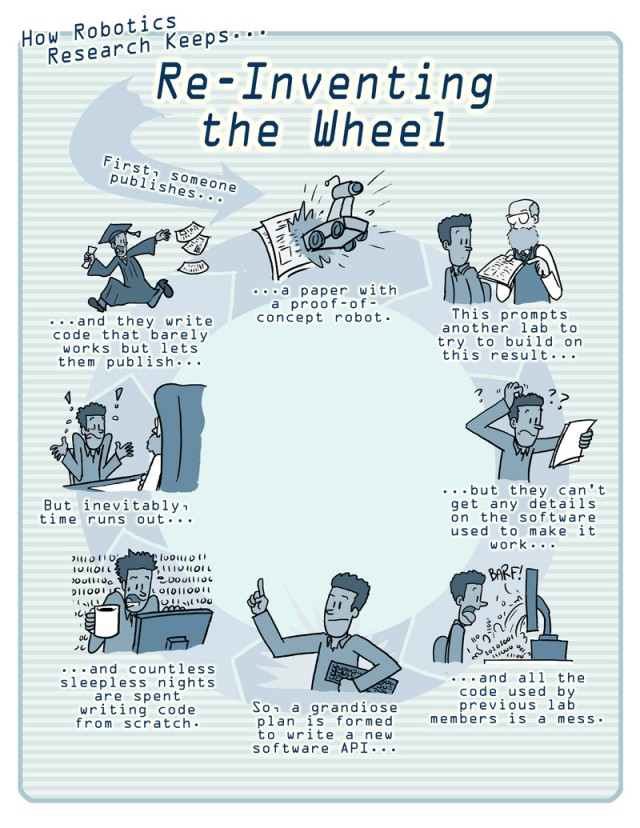
\includegraphics[width=.66\linewidth]{figures/stop_reinventing_theWheel.jpg}
    
\tiny{http://www.willowgarage.com/blog/2010/04/27/reinventing-wheel}
\end{frame}


\begin{frame}{What ROS is}
    \framesubtitle{Robot Operating System}
    \begin{itemize}
        \item A way to standardize writing software for robots.
        \item It enhances {\huge code reusability} 
\includegraphics[scale=0.02]{figures/recycling.png}.
        \item ROS is open-source 
\includegraphics[scale=0.09]{figures/open_source.png}.
        \item It is a meta-operating system.
        \item ROS can be installed on Ubuntu and Debian (so it’s currently supported on Linux only).
        
        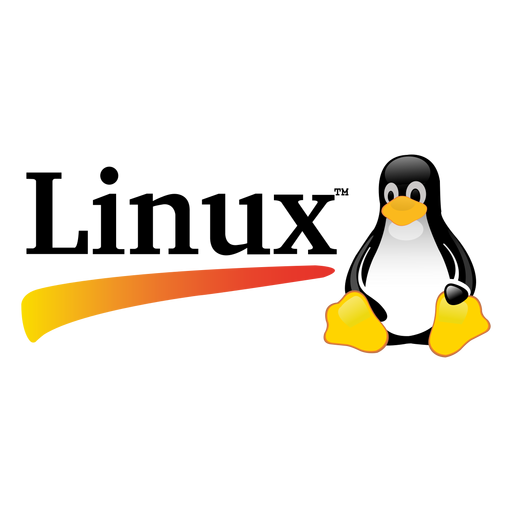
\includegraphics[width=.1\linewidth]{figures/linux_logo.png}
        
\includegraphics[width=.1\linewidth]{figures/ubuntu_logo.png} 
        
\includegraphics[width=.06\linewidth]{figures/debian_logo.png} 
    \end{itemize}
\end{frame}


\subsection{What ROS is NOT}
\begin{frame}{What ROS is NOT}
    \framesubtitle{Robot Operating System}
    \begin{itemize}
        \item It is NOT a programming language.
        \item It is NOT an integrated development environment
        (IDE).
        \item It is NOT a stand-alone operating system 
    \end{itemize}
\end{frame}


%---------------------------

\section{Analogy Between ROS and Operating Systems}

\begin{frame}{Analogy Between ROS and Operating Systems}
    \begin{overpic}[width=.45\linewidth]{figures/analogy1.png}
        \put (130,80) {Software Applications}
        \put (130,50) {work on}
        \put (130,20) {Different hardware}        
    \end{overpic}
\end{frame}

\begin{frame}{Analogy Between ROS and Operating Systems}
    \centering
    \begin{overpic}[width=.4\linewidth]{figures/analogy2.png}
        \put (35,90) {Application} 
        \put (9,65) {\footnotesize Operating System} 
        \put (12,43) {\footnotesize Device Drivers}   
    \end{overpic}
\end{frame}

\begin{frame}{Analogy Between ROS and Operating Systems}
    \centering
    \begin{overpic}[width=.3\linewidth]{figures/analogy3.png}
        \put (2,102) {Mapping algorithm}
        \put (21.5,74) {ROS} 
        \put (11,49) {Laser driver} 
        \put (-25,10) {Laser scanner} 
    \end{overpic}
\end{frame}


\begin{frame}{Analogy Between ROS and Operating Systems}
    \centering
    \begin{overpic}[width=.8\linewidth]{figures/analogy4.png}
        \put (34,72) {Mapping algorithm}
        \put (46.5,54) {ROS}
        \put (2.3,29) {Laser driver}
        \put (38,29) {Laser driver}
        \put (75,29) {Laser driver}
    \end{overpic}
\end{frame}

\begin{frame}{Analogy Between ROS and Operating Systems}
    \begin{overpic}[width=.8\linewidth]{figures/analogy4.png}
        \put (34,72) {Mapping algorithm}
        \put (46.5,54) {ROS}
        \put (2.3,29) {Laser driver}
        \put (38,29) {Laser driver}
        \put (75,29) {Laser driver}
    \end{overpic}
\end{frame}

\begin{frame}{Analogy Between ROS and Operating Systems}
    \begin{overpic}[width=.8\linewidth]{figures/analogy5.png}
        \put (34,72) {Mapping algorithm}
        \put (46.5,54) {ROS}
        \put (2.3,29) {Laser driver}
        \put (38,29) {Laser driver}
        \put (75,29) {Laser driver}
        \put (105,10) {\footnotesize Different hardware}
    \end{overpic}
\end{frame}

\begin{frame}{Analogy Between ROS and Operating Systems}
    \begin{overpic}[width=.8\linewidth]{figures/analogy6.png}
        \put (34,72) {Mapping algorithm}
        \put (46.5,54) {ROS}
        \put (2.3,29) {Laser driver}
        \put (38,29) {Laser driver}
        \put (75,29) {Laser driver}
        \put (105,10) {\footnotesize Different hardware}
        \put (105,30) {\footnotesize Different drivers}
    \end{overpic}
\end{frame}

\begin{frame}{Analogy Between ROS and Operating Systems}
    \begin{overpic}[width=.8\linewidth]{figures/analogy7.png}
        \put (34,72) {Mapping algorithm}
        \put (46.5,54) {ROS}
        \put (2.3,29) {Laser driver}
        \put (38,29) {Laser driver}
        \put (75,29) {Laser driver}
        \put (105,10) {\footnotesize Different hardware}
        \put (105,30) {\footnotesize Different drivers}        
        \put (105,58) {\footnotesize Data received in}
        \put (105,54) {\footnotesize the same message}
        \put (105,50) {\footnotesize format}
    \end{overpic}
\end{frame}

\begin{frame}{Analogy Between ROS and Operating Systems}
    \begin{overpic}[width=.8\linewidth]{figures/analogy7.png}
        \put (34,72) {Mapping algorithm}
        \put (46.5,54) {ROS}
        \put (2.3,29) {Laser driver}
        \put (38,29) {Laser driver}
        \put (75,29) {Laser driver}
        \put (105,10) {\footnotesize Different hardware}
        \put (105,30) {\footnotesize Different drivers}        
        \put (105,58) {\footnotesize Data received in}
        \put (105,54) {\footnotesize the same message}
        \put (105,50) {\footnotesize format}
        \put (105,72) {\footnotesize No change}
    \end{overpic}
\end{frame}

\begin{frame}{Analogy Between ROS and Operating Systems}
    \begin{overpic}[width=.45\linewidth]{figures/analogy8.png}
        \put (130,77) {Robot Applications}
        \put (3,75) {\scriptsize Mapping}
        \put (33,75) {\scriptsize Navigation}
        \put (66,75) {\scriptsize pick \& place}
        \put (130,50) {work on}
        \put (130,20) {Different hardware}        
    \end{overpic}
\end{frame}

\begin{frame}[label=figs2]{Analogy Between ROS and Operating Systems}
\centering
 \scalebox{0.9}{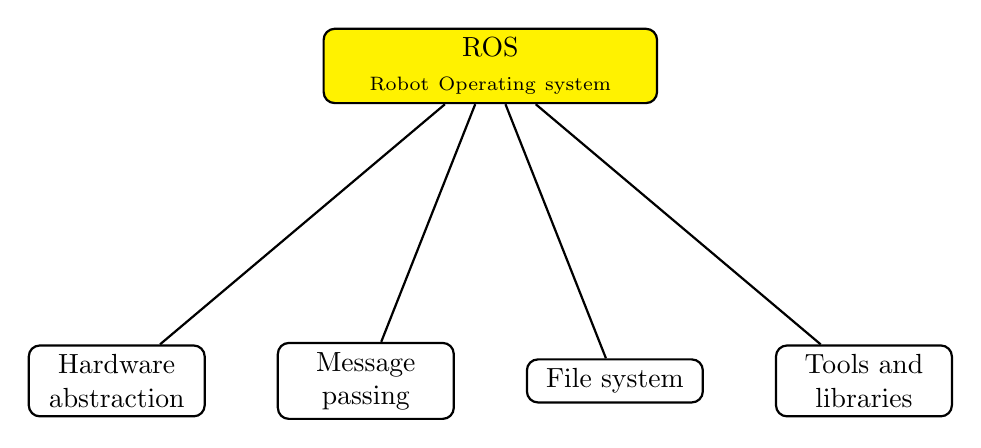
\begin{tikzpicture}[sibling distance=9em, level distance = 4.0cm, thick,
every node/.style = {shape=rectangle, rounded corners,
    draw, align=center}]]
\node [text width=4cm, fill = yellow]{ROS \\ \scriptsize Robot Operating system}
child { node [text width=2cm]{Hardware abstraction} }
child { node [text width=2cm]{Message passing} }
child { node [text width=2cm]{File system} }
child { node [text width=2cm]{Tools and libraries} };
\end{tikzpicture}}
\end{frame}





%---------------------------

\section{Features of ROS}

\begin{frame}{Features of ROS}

\begin{itemize}
        \item Language independent.
        \item Distributed and Modular.
        \item A lot of libraries and tools.
        \item Open Source.
        \item Active Community.
\end{itemize}
\end{frame}

\subsection{Language independent}
\begin{frame}{Features of ROS}
\framesubtitle{Language independent}    
\begin{itemize}
    \item ROS functionalities are implemented as a library in different programming languages.
    \item  These libraries are referred to as ROS client libraries.
\end{itemize}
\end{frame}

\begin{frame}{Language independent}
    \framesubtitle{Features of ROS}    

    ROS client libraries.  
    
    \vspace{0.5cm}
    \centering
\scalebox{0.8}{%
  \begin{minipage}{\textwidth}
    \begin{itemize}
        \item Main ROS Client libraries:
        \begin{itemize}
            \item roscpp \hspace{7cm} 
\includegraphics[width=.06\linewidth]{figures/cpp_logo.png}
            \item rospy  \hspace{7.1cm} 
\includegraphics[width=.08\linewidth]{figures/python_logo.png}
            \item roslisp \hspace{7cm} 
\includegraphics[width=.06\linewidth]{figures/lisp_logo.png}
        \end{itemize}
        \item Experimental ROS client libraries:
        \begin{itemize}
            \item rosjava \hspace{7cm} 
\includegraphics[width=.06\linewidth]{figures/java_logo.png}
            \item rosruby \hspace{7cm} 
\includegraphics[width=.06\linewidth]{figures/ruby_logo.png}
            \item and some others..
        \end{itemize}
        \item ROS support on MATLAB:
        \begin{itemize}
            \item Robotics System Toolbox \hspace{4.3cm} 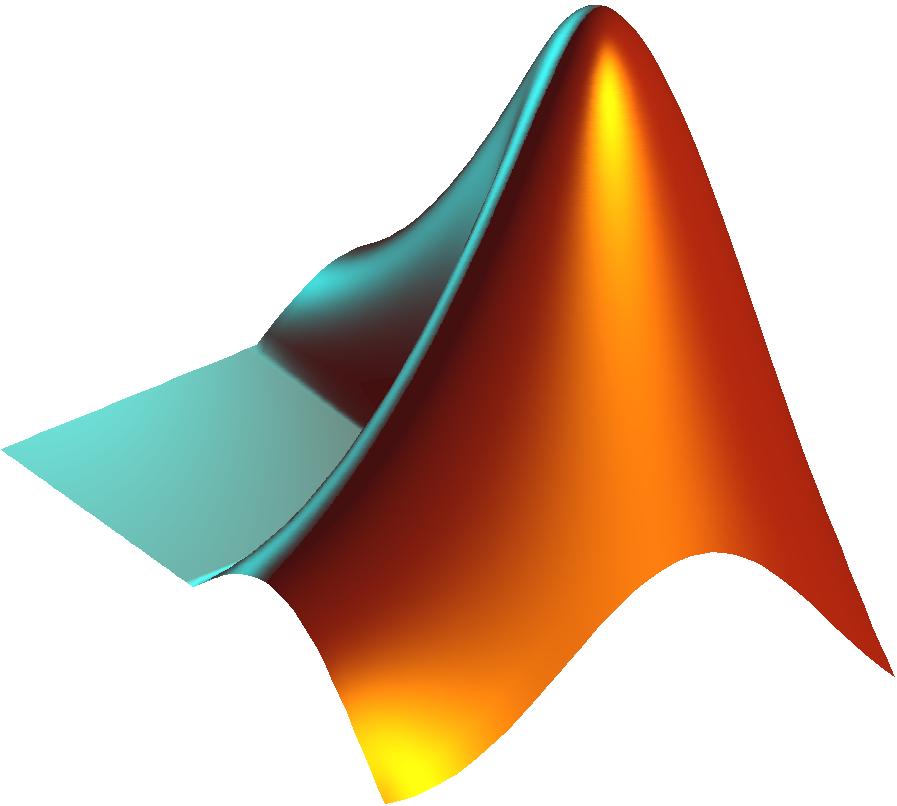
\includegraphics[width=.06\linewidth]{figures/matlab_logo.png}
        \end{itemize}
    \end{itemize}
\end{minipage}%
}
\end{frame}


\subsection{Distributed and Modular}

\begin{frame}{Distributed and Modular}
    \framesubtitle{Features of ROS}    
    \begin{itemize}
        \item ROS supports running processes on multiple computers connected together through a LAN.
        \item In a system running ROS, there will be multiple of processes where each process can do
        certain task. A process can be changed without altering the remaining processes.
    \end{itemize}
\end{frame}


\subsection{A lot of libraries and tools}

\begin{frame}{A lot of libraries and tools}
    \framesubtitle{Features of ROS}    
    \begin{itemize}
        \item Examples of libraries:
            \begin{itemize}
                \item Navigation stack.
                \item SLAM (gmapping, hector SLAM, etc..).
                \item Localization (amcl, etc..).
                \item Motion planning for manipulators (MoveIt)
                \item Support for popular libraries (OpenCV, PCL).
            \end{itemize}
            
        \item Examples of tools:
            \begin{itemize}
                \item RVIZ:3D Visualization.
                \item ROS bag files: Logging Sensor Data.
                \item Catkin: A Build System.
                \item Command line tools.
            \end{itemize}        
    \end{itemize}
\end{frame}


\subsection{Bad Things About ROS}

\begin{frame}{Bad Things About ROS}
            \begin{itemize}
                \item Learning ROS needs time. 
                \item It needs a computer. Does not work on a microcontroller!
                \item Not optimized for multiple robots.
                \item Supported only on Linux, no support for Windows or macOS.
            \end{itemize}  
\end{frame}





%---------------------------

\section{ROS Concepts}

\begin{frame}{ROS Concepts}
\tikzstyle{every node}=[draw=white,thick,anchor=west]
\tikzstyle{selected}=[draw=red,fill=red!30]
\tikzstyle{optional}=[dashed,fill=gray!50]
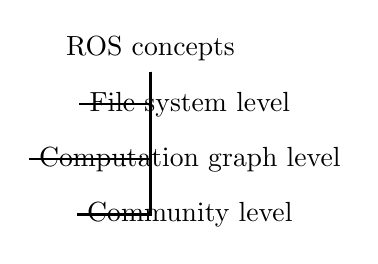
\begin{tikzpicture}[%
thick, grow via three points={one child at (0.5,-0.7) and
    two children at (0.5,-0.7) and (0.5,-1.4)},
edge from parent path={(\tikzparentnode.south) |- (\tikzchildnode.west)}]
\node {ROS concepts}
child { node {File system level}}		
child { node {Computation graph level}}
child { node {Community level}};
\end{tikzpicture}
\end{frame}


\subsection{File system level}

\begin{frame}{File system level}
  \framesubtitle{ROS Concepts}
    
 \centering
 \scalebox{0.9}{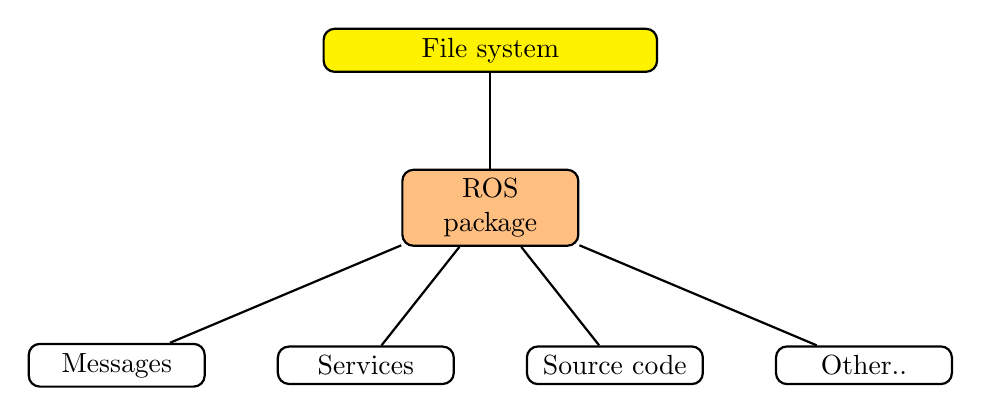
\begin{tikzpicture}[sibling distance=9em, level distance = 2.0cm, thick,
     every node/.style = {shape=rectangle, rounded corners,
         draw, align=center}]]
        \node [text width=4cm, fill = yellow]{File system}
         child { node [text width=2cm, fill = orange!50]{ROS package} 
        child { node [text width=2cm]{Messages} }
        child { node [text width=2cm]{Services} }
        child { node [text width=2cm]{Source code} }
        child { node [text width=2cm]{Other..} }
        };
        \end{tikzpicture}}
\end{frame}


\begin{frame}{File system level}
    \framesubtitle{ROS Concepts}
    
    \centering
    \scalebox{0.9}{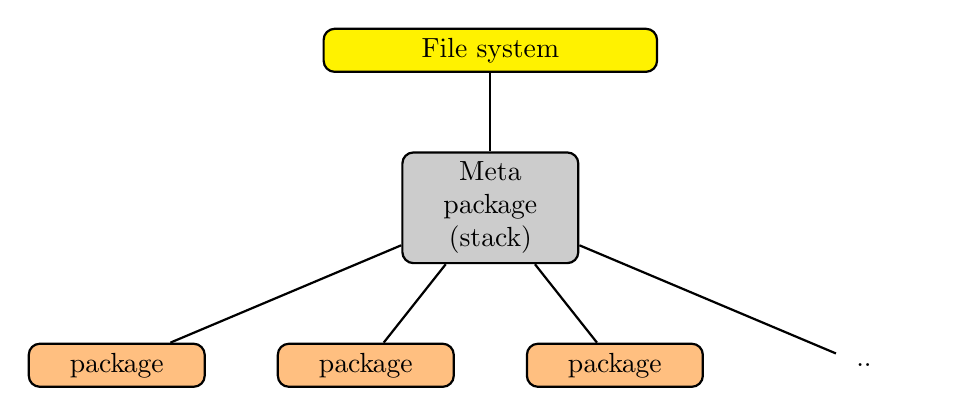
\begin{tikzpicture}[sibling distance=9em, level distance = 2.0cm, thick,
        every node/.style = {shape=rectangle, rounded corners,
            draw, align=center}]]
        \node [text width=4cm, fill = yellow]{File system}
        child { node [text width=2cm, fill = black!20]{Meta package \\ (stack)} 
            child { node [text width=2cm, fill = orange!50]{package} }
            child { node [text width=2cm, fill = orange!50]{package} }
            child { node [text width=2cm, fill = orange!50]{package} }
            child { node [text width=2cm, fill = none, draw = none]{..} }
        };
        \end{tikzpicture}}
\end{frame}


\begin{frame}{File system level}
    \framesubtitle{ROS Concepts}
Inside a ROS package:

\vspace{0.5cm}
\centering
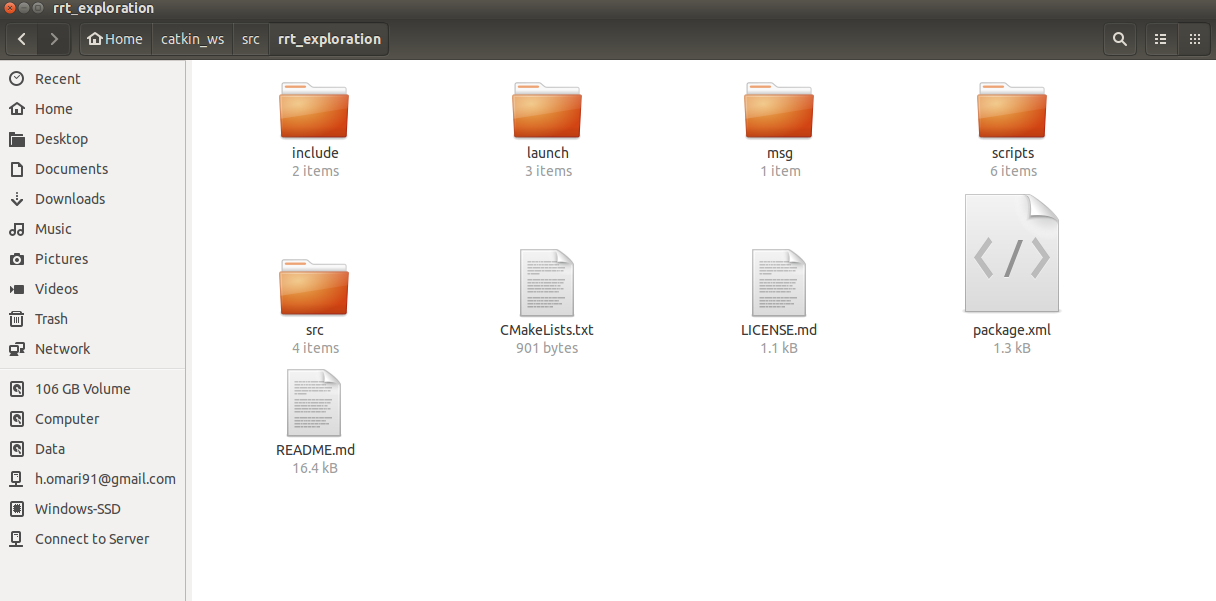
\includegraphics[width=.9\linewidth]{figures/example_package.png}
\end{frame}

    
\subsection{Computation graph level}

\begin{frame}{Computation graph level}
    \framesubtitle{ROS Concepts}
    \begin{itemize}
        \item In an application that uses ROS, the computations are executed by a collection of processes called Nodes.
        \item Nodes are connected together in a peer-to-peer network.
        \item This network of nodes do all the computation and is referred to as ROS computation graph.
        \item ROS Nodes can be run on single or multiple computers.
    \end{itemize}
\end{frame}

\begin{frame}{Computation graph level}
    \framesubtitle{ROS Concepts}
    
    Concepts related to ROS computation graph:
    
    \begin{enumerate}
        \item Nodes.
        \item Topics.
        \item Messages.
        \item Master.
        \item Parameter Server.
        \item Services.
        \item Bags.
    \end{enumerate}
\end{frame}

\begin{frame}{Computation graph level}
    \framesubtitle{ROS Concepts}
    {\huge Nodes:}
    \vspace{1cm}
    \begin{itemize}
        \item A ROS node is a process that exchanges data with other processes through ROS network.
        
        \item It may be a python script, a C++ written process, or even a MATLAB script.
        
        \item Nodes perform computation.
    \end{itemize}
\end{frame}

 \begin{frame}[plain]{}
     \begin{textblock}{5}(5,10)
         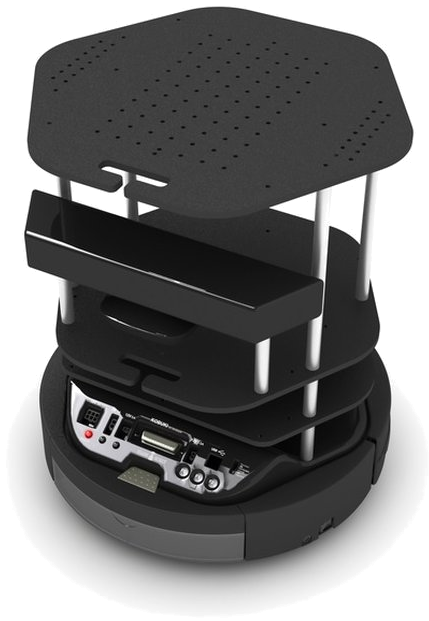
\includegraphics[width=0.5\linewidth]{figures/platform.png}
     \end{textblock}
    \end{frame}
    
     \begin{frame}[plain]{}
         \begin{textblock}{5}(5,10)
             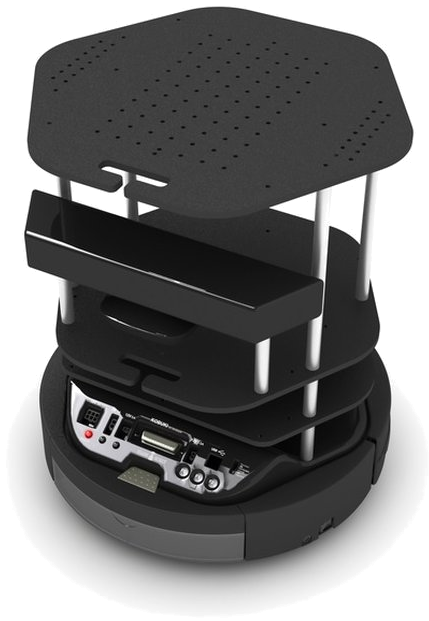
\includegraphics[width=0.5\linewidth]{figures/platform.png}
            \end{textblock}
         \begin{textblock}{5}(4,5.2)
             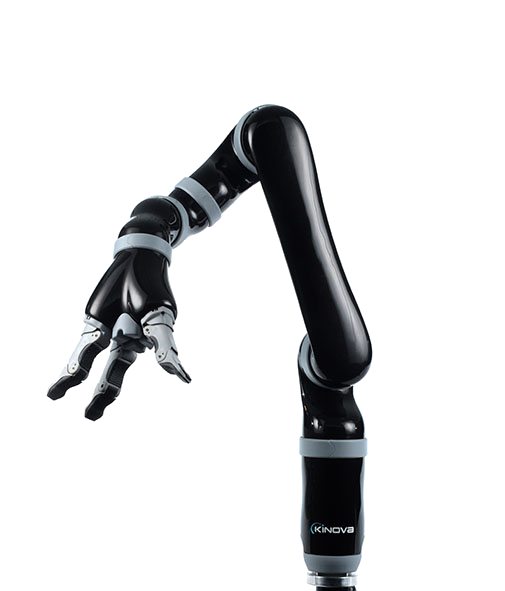
\includegraphics[width=0.7\linewidth]{figures/robot_arm.png}
            \end{textblock}
          \begin{textblock}{5}(0,5)
              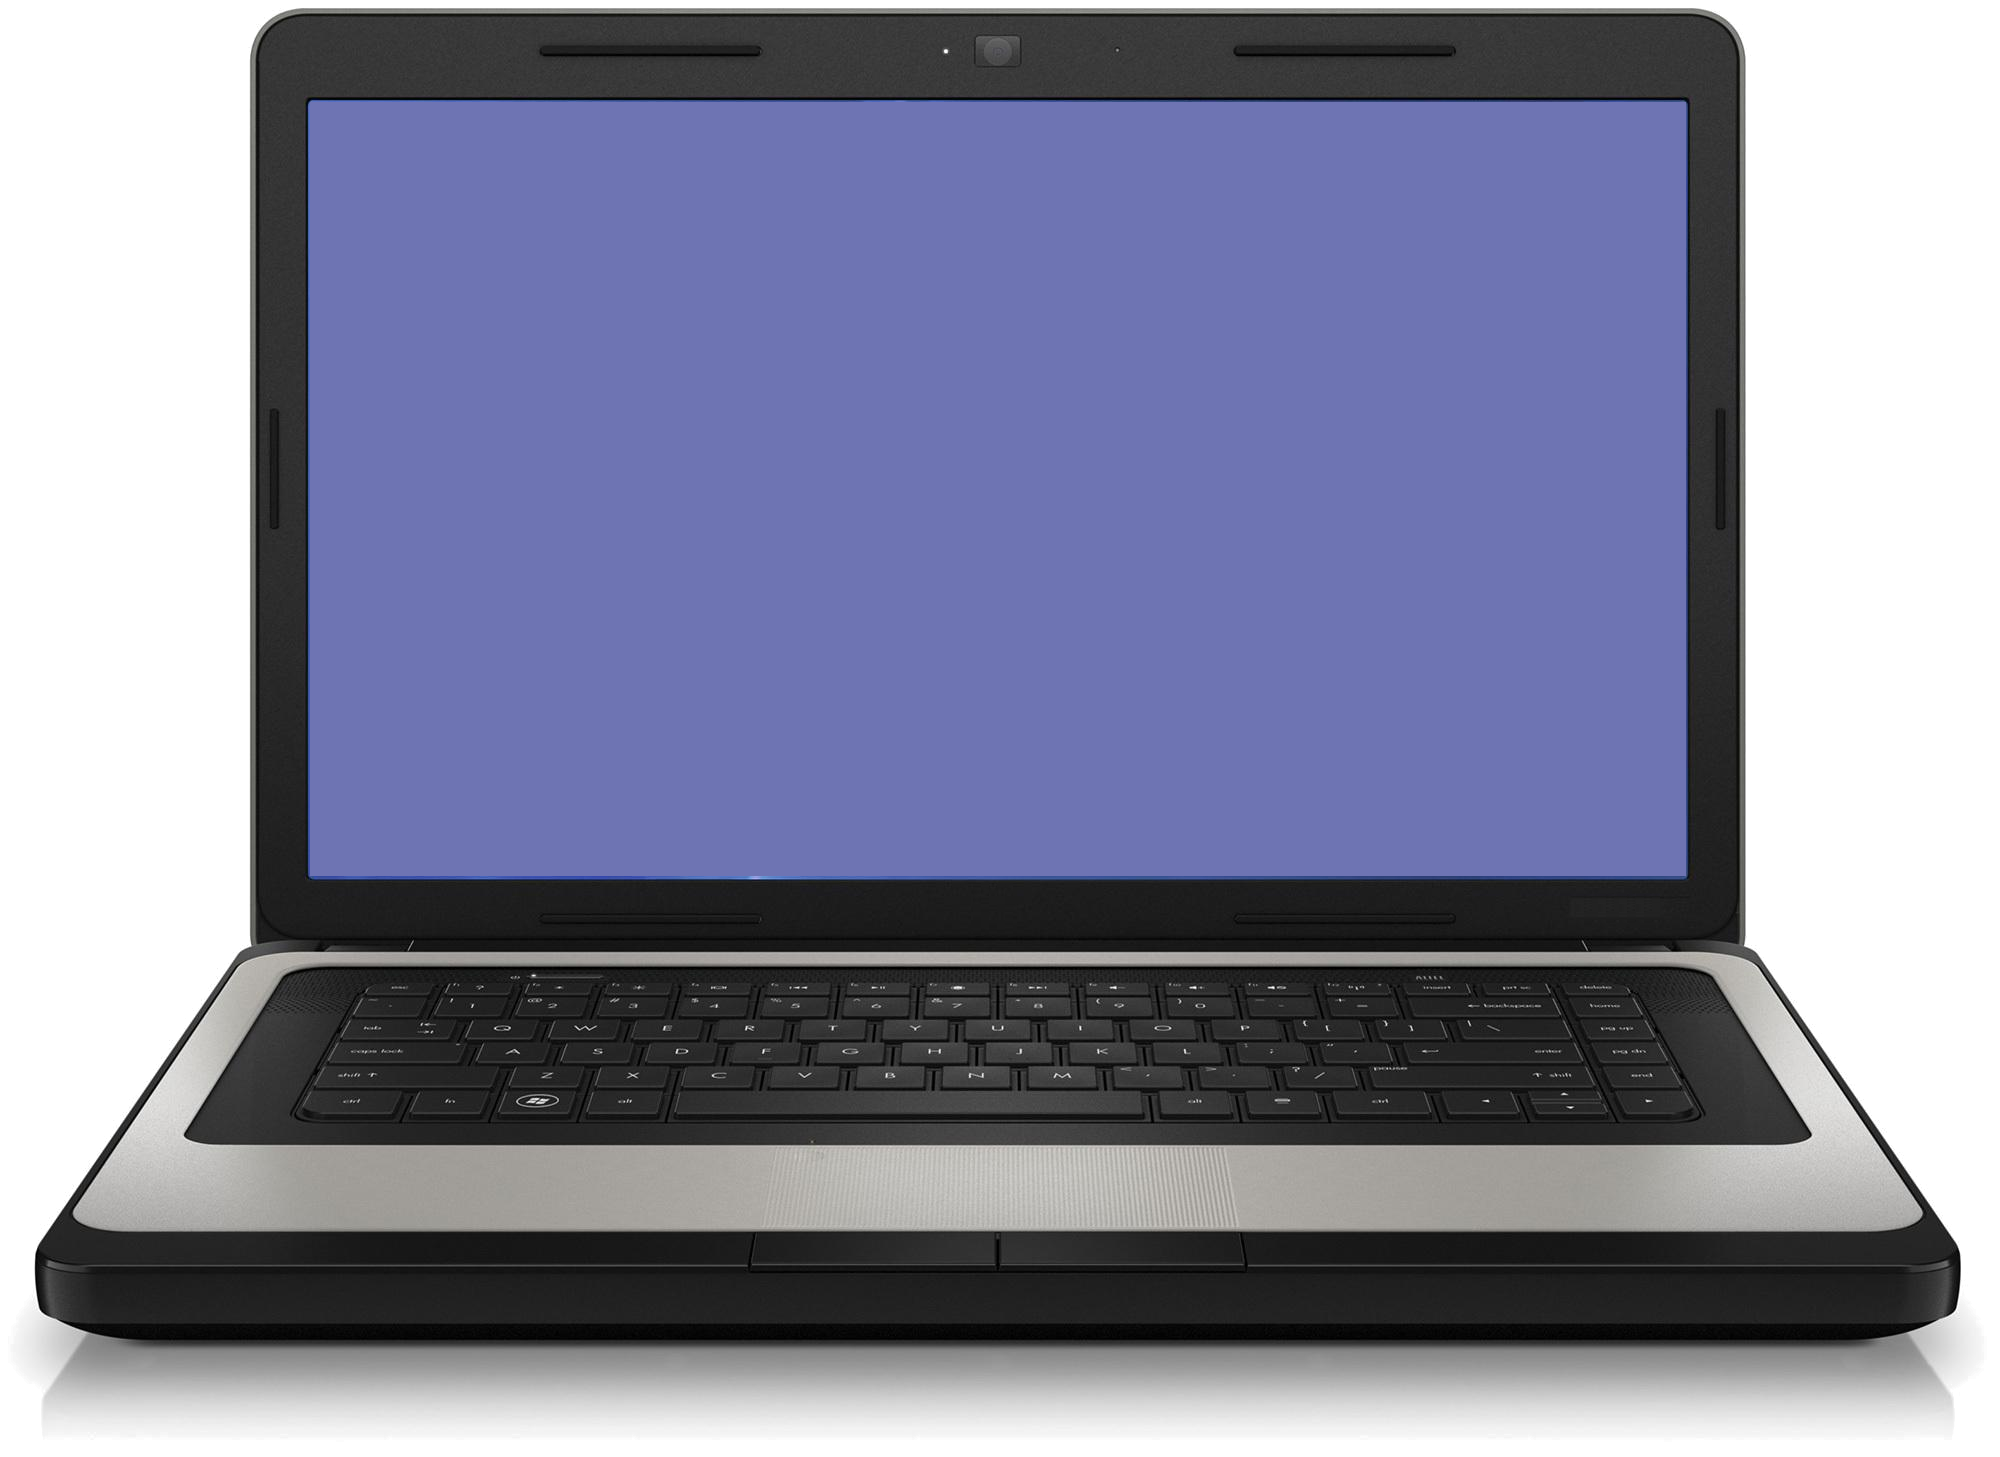
\includegraphics[width=0.6\linewidth]{figures/laptop.png}
            \end{textblock} 
        \end{frame}
        
         \begin{frame}[plain]{}
             \begin{textblock}{5}(5,10)
                 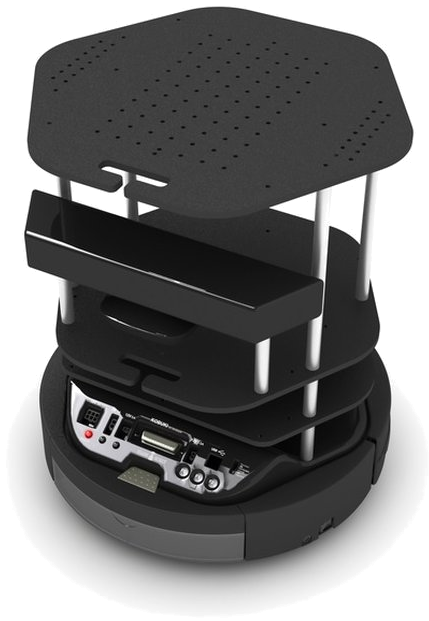
\includegraphics[width=0.5\linewidth]{figures/platform.png}
                \end{textblock}
                \begin{textblock}{5}(4,5.2)
                    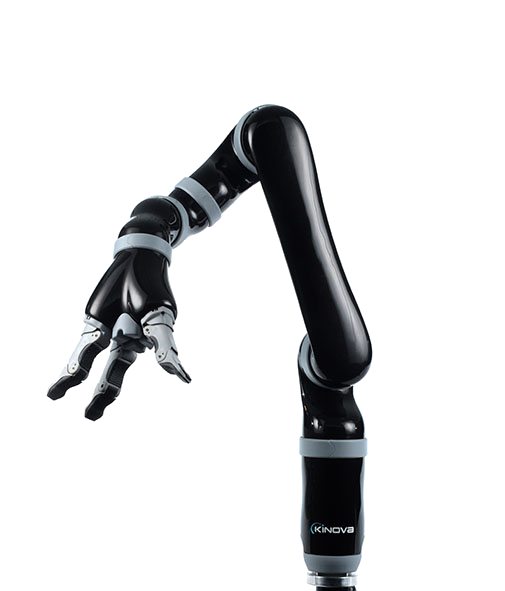
\includegraphics[width=0.7\linewidth]{figures/robot_arm.png}
                \end{textblock}
                \begin{textblock}{5}(9.5,8)
                    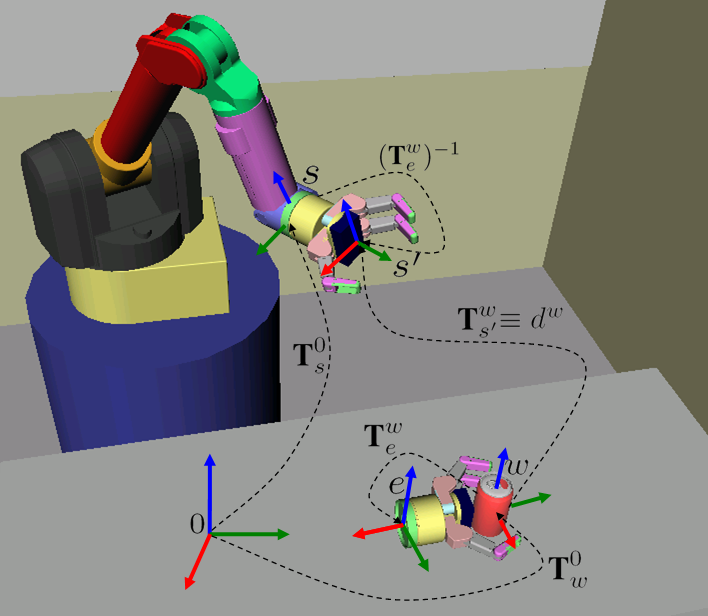
\includegraphics[width=1.2\linewidth]{figures/pick_and_place.png}
                \end{textblock}                
          \begin{textblock}{5}(0,5)
              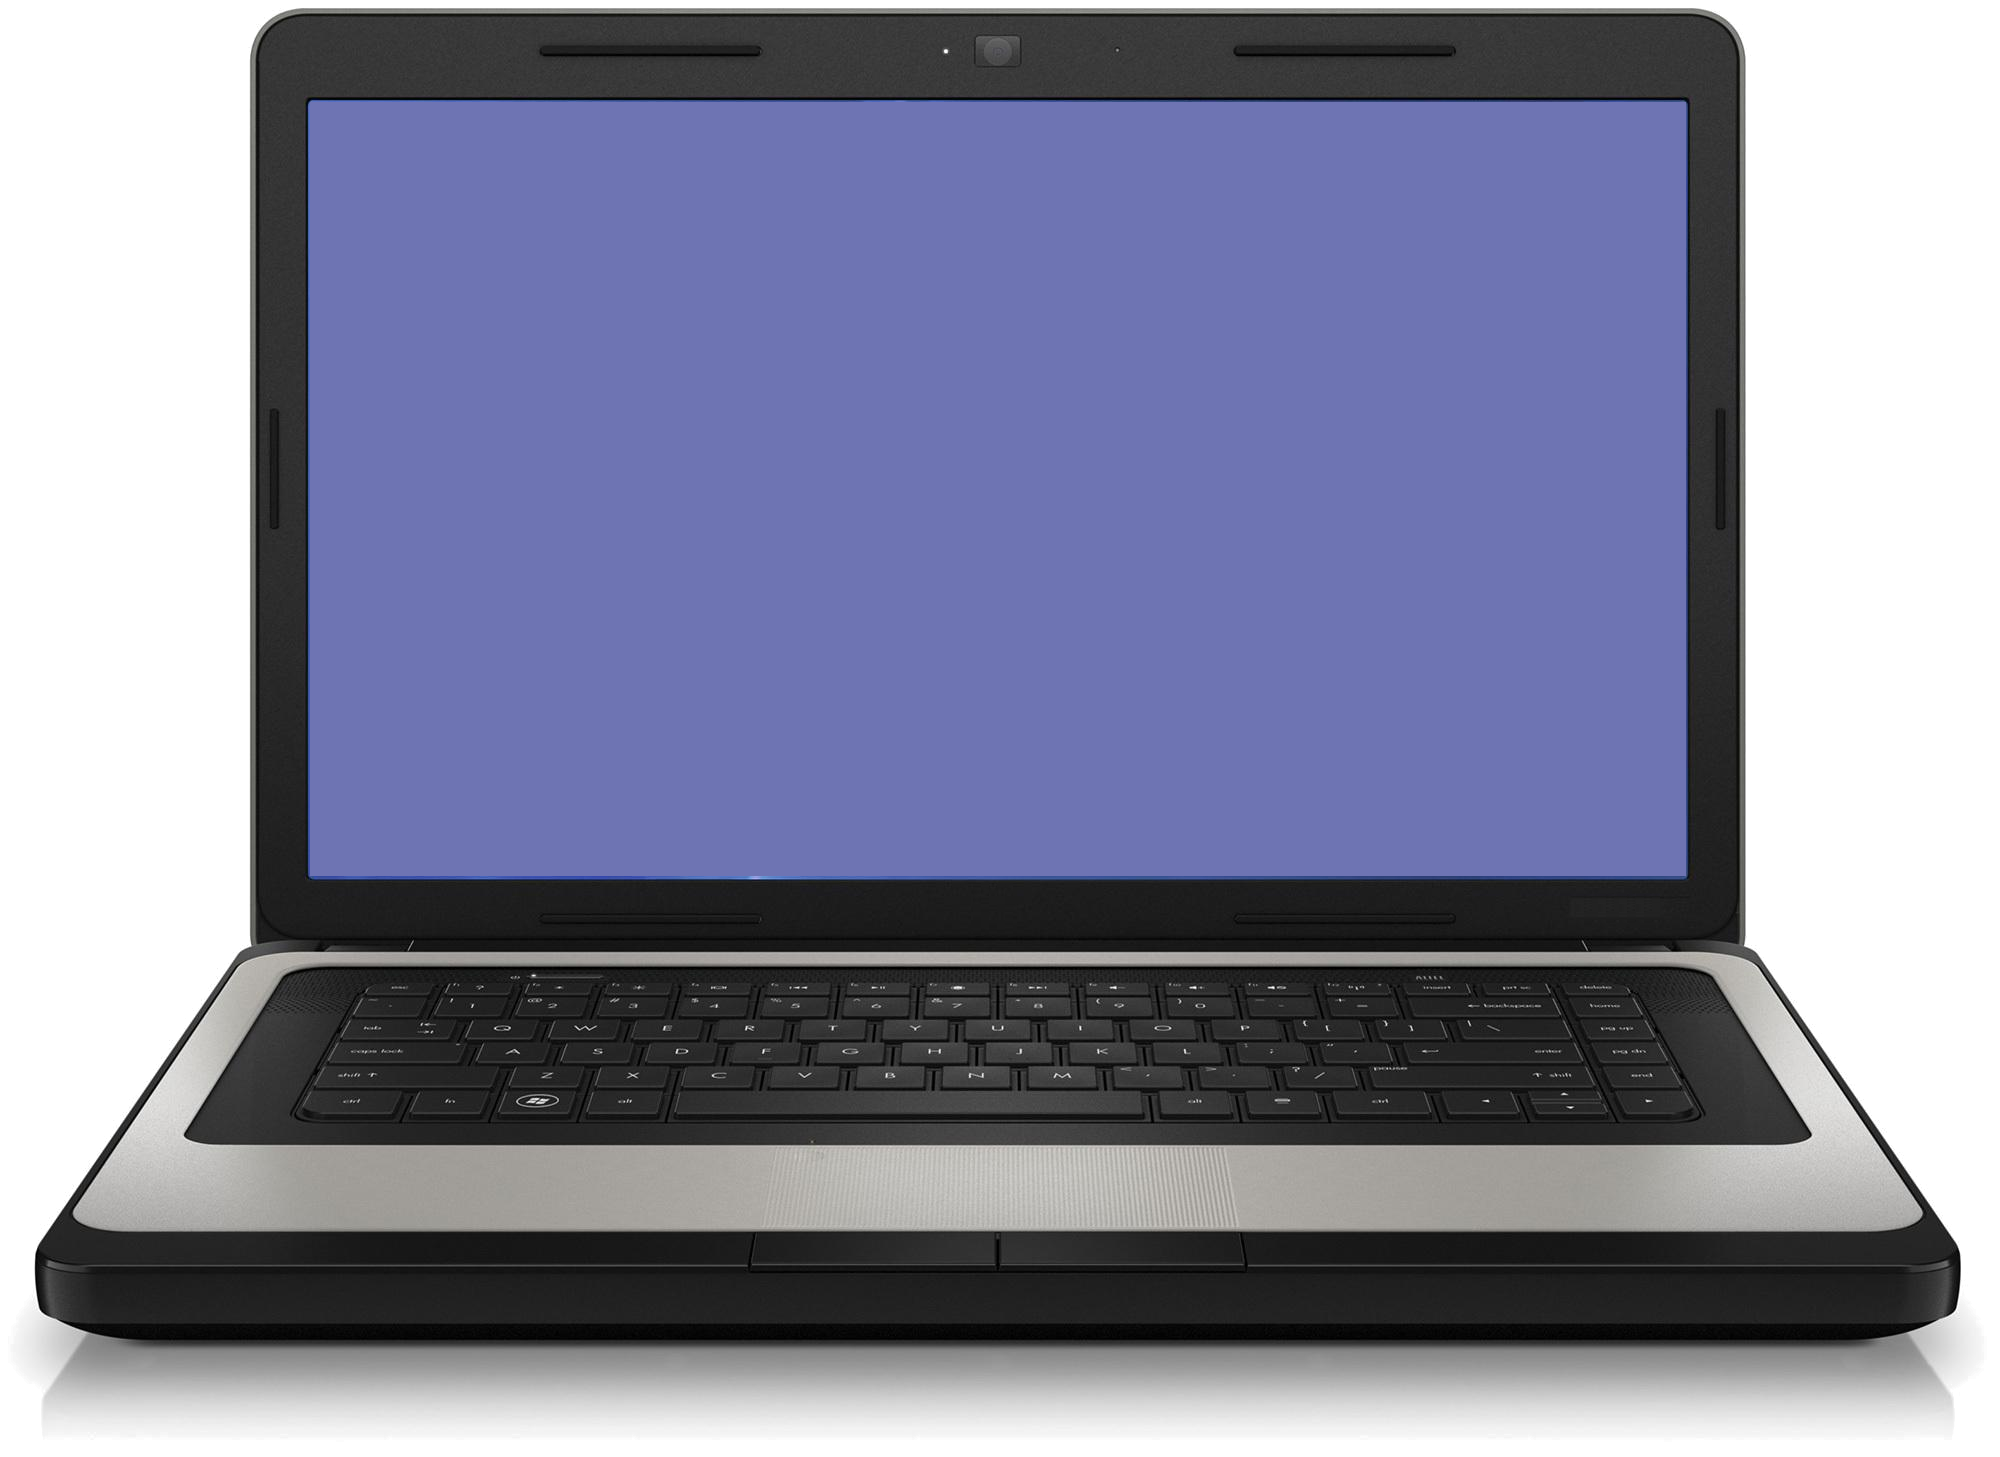
\includegraphics[width=0.6\linewidth]{figures/laptop.png}
            \end{textblock} 
            \end{frame}
        
     \begin{frame}[plain]{}
         \begin{textblock}{5}(5,10)
             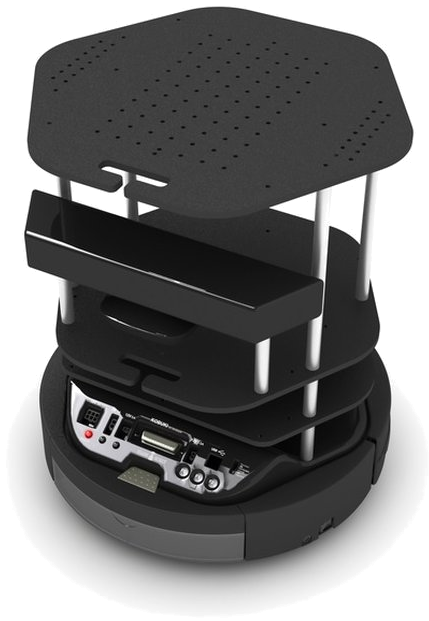
\includegraphics[width=0.5\linewidth]{figures/platform.png}
            \end{textblock}
            \begin{textblock}{5}(4,5.2)
                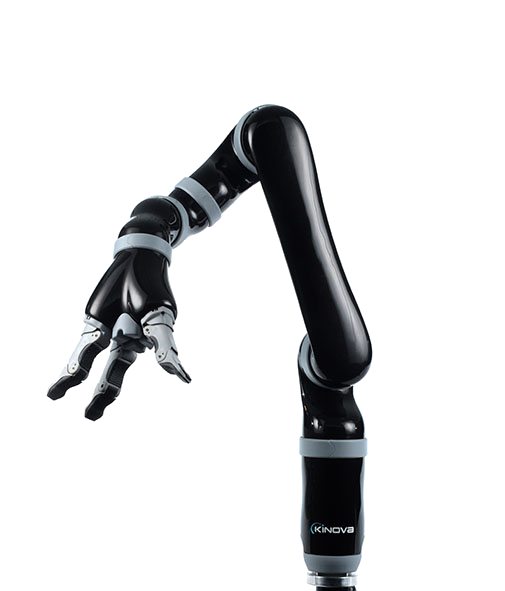
\includegraphics[width=0.7\linewidth]{figures/robot_arm.png}
            \end{textblock}
            \begin{textblock}{5}(5,1.5)
                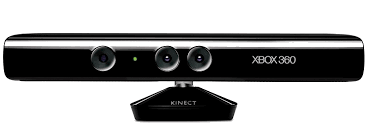
\includegraphics[width=0.6\linewidth]{figures/kinect.png}
            \end{textblock}  
                \begin{textblock}{5}(9.5,8)
                    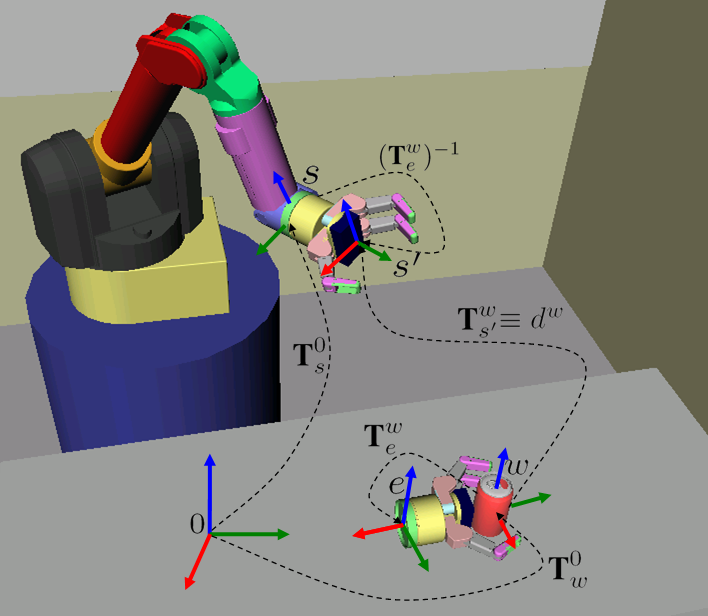
\includegraphics[width=1.2\linewidth]{figures/pick_and_place.png}
                  \end{textblock}                      
          \begin{textblock}{5}(0,5)
              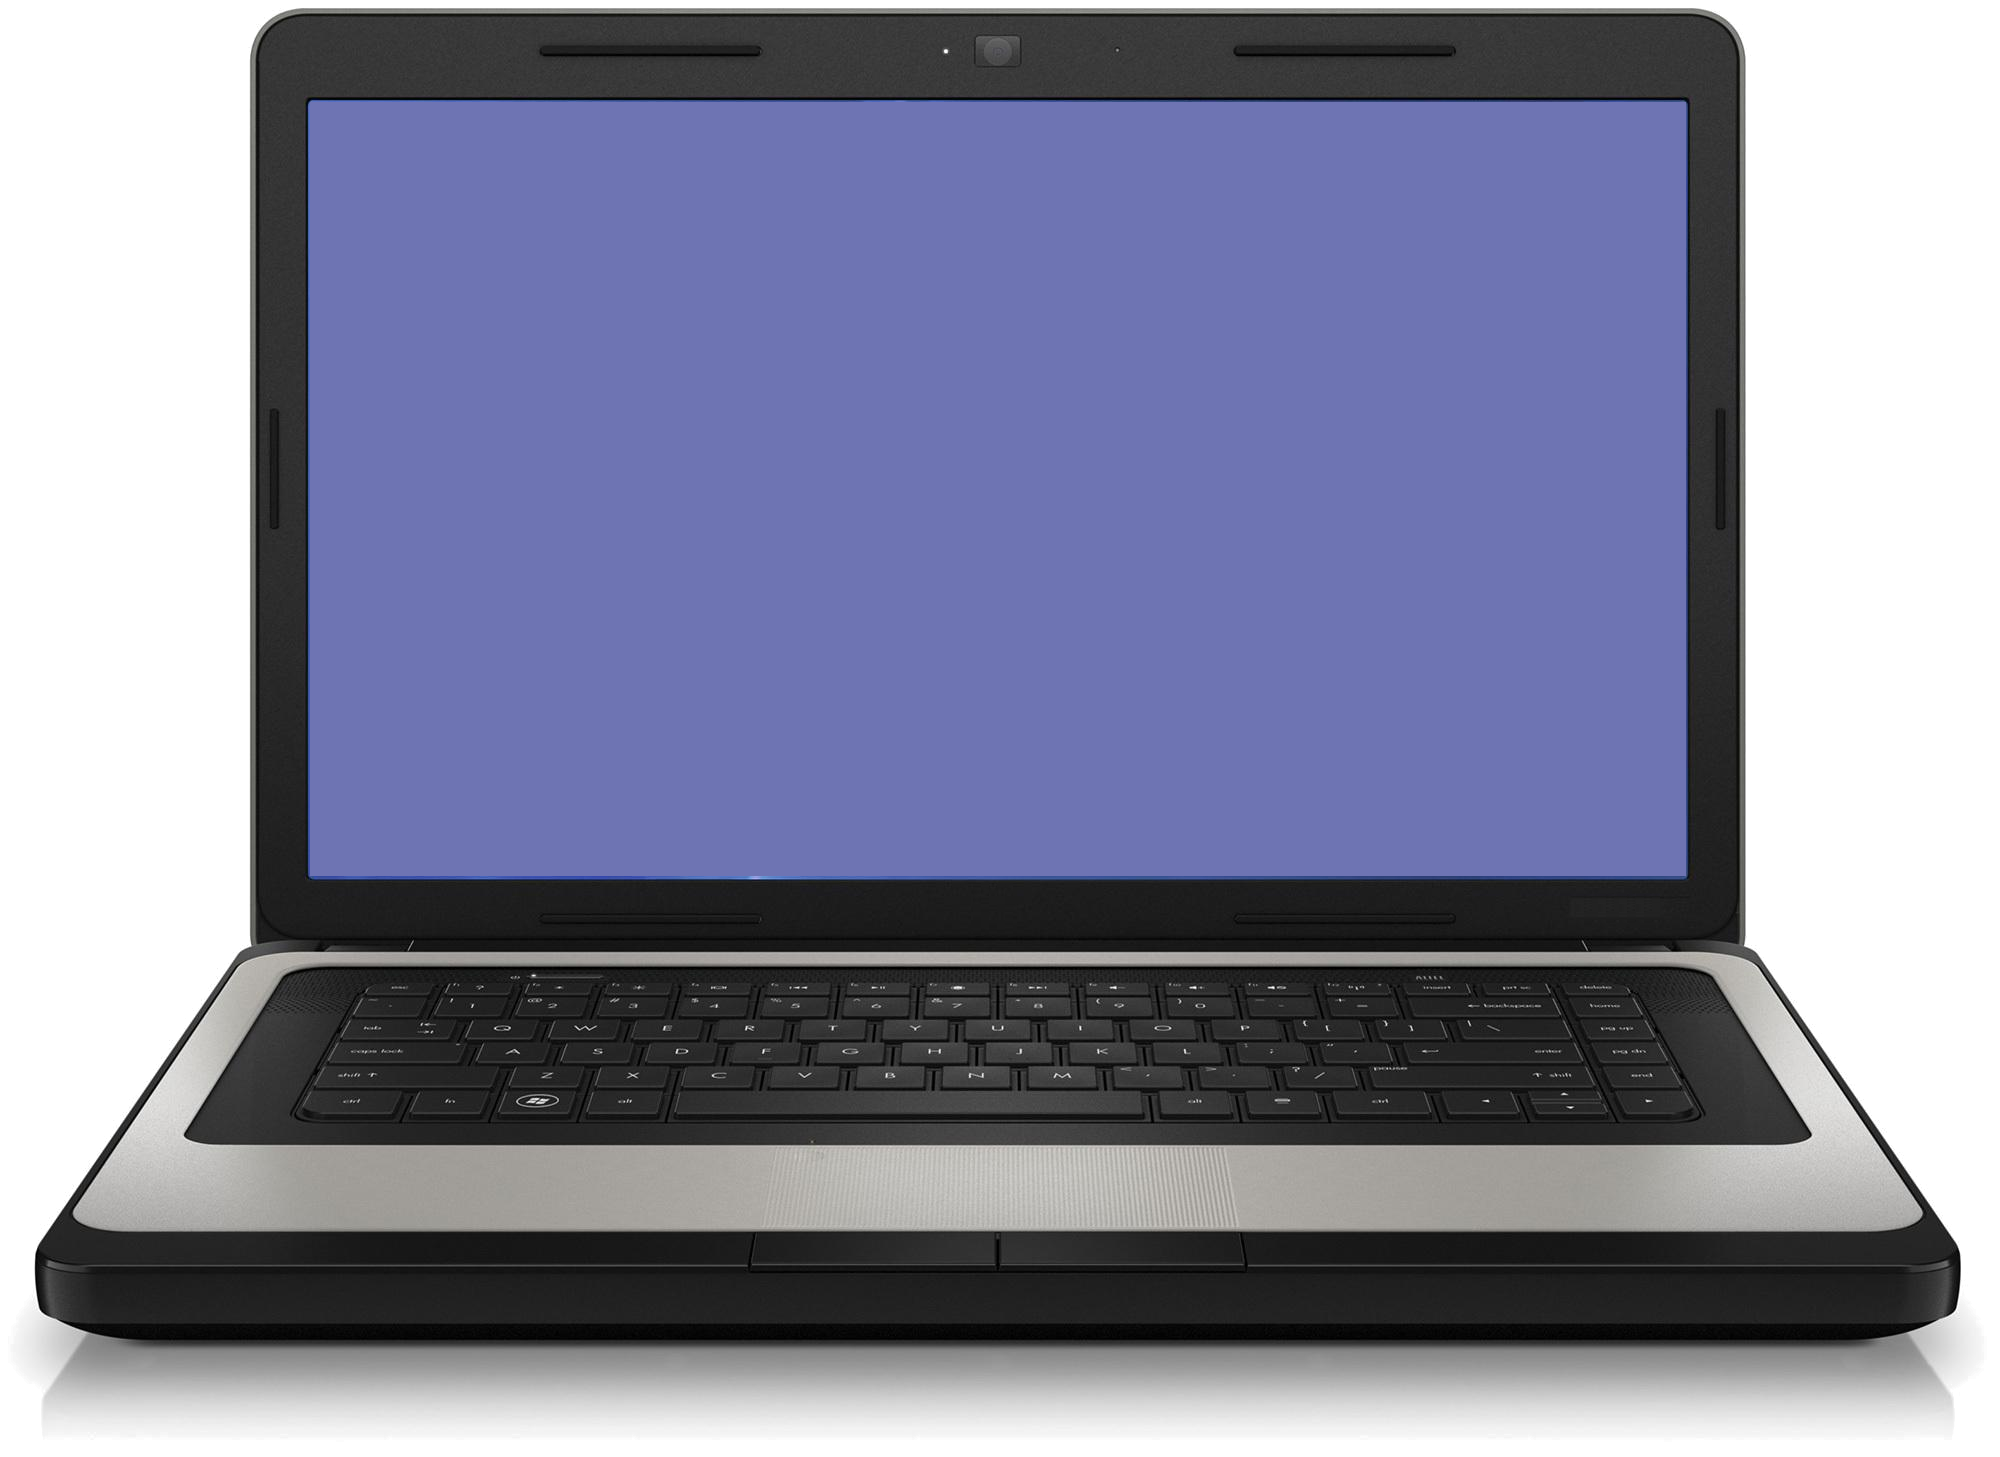
\includegraphics[width=0.6\linewidth]{figures/laptop.png}
            \end{textblock} 
        \end{frame}  


      
     \begin{frame}[plain]{}
         \begin{textblock}{5}(5,10)
             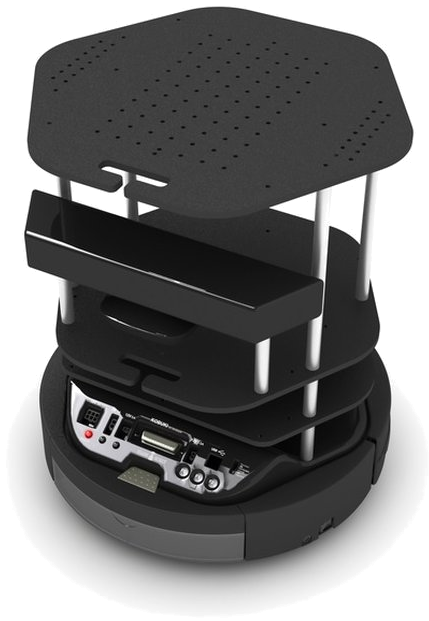
\includegraphics[width=0.5\linewidth]{figures/platform.png}
           \end{textblock}
           \begin{textblock}{5}(4,5.2)
               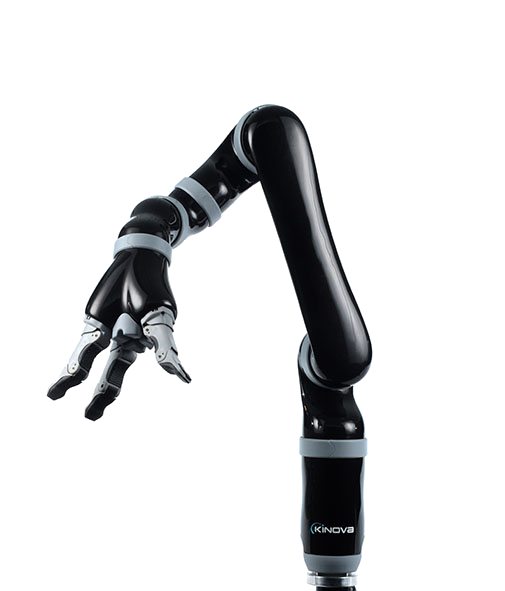
\includegraphics[width=0.7\linewidth]{figures/robot_arm.png}
           \end{textblock}
           \begin{textblock}{5}(5,1.5)
               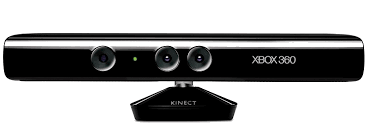
\includegraphics[width=0.6\linewidth]{figures/kinect.png}
           \end{textblock} 
                \begin{textblock}{5}(9.5,8)
                    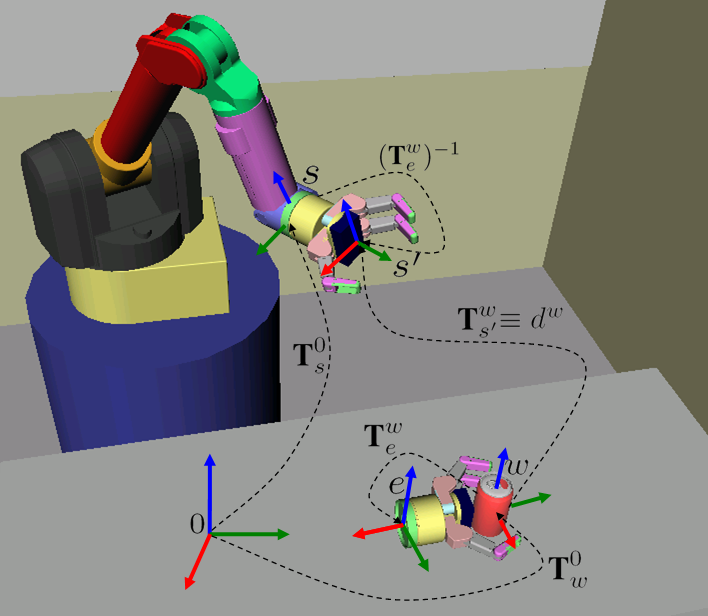
\includegraphics[width=1.2\linewidth]{figures/pick_and_place.png}
                 \end{textblock}           
           \begin{textblock}{5}(0,5)
               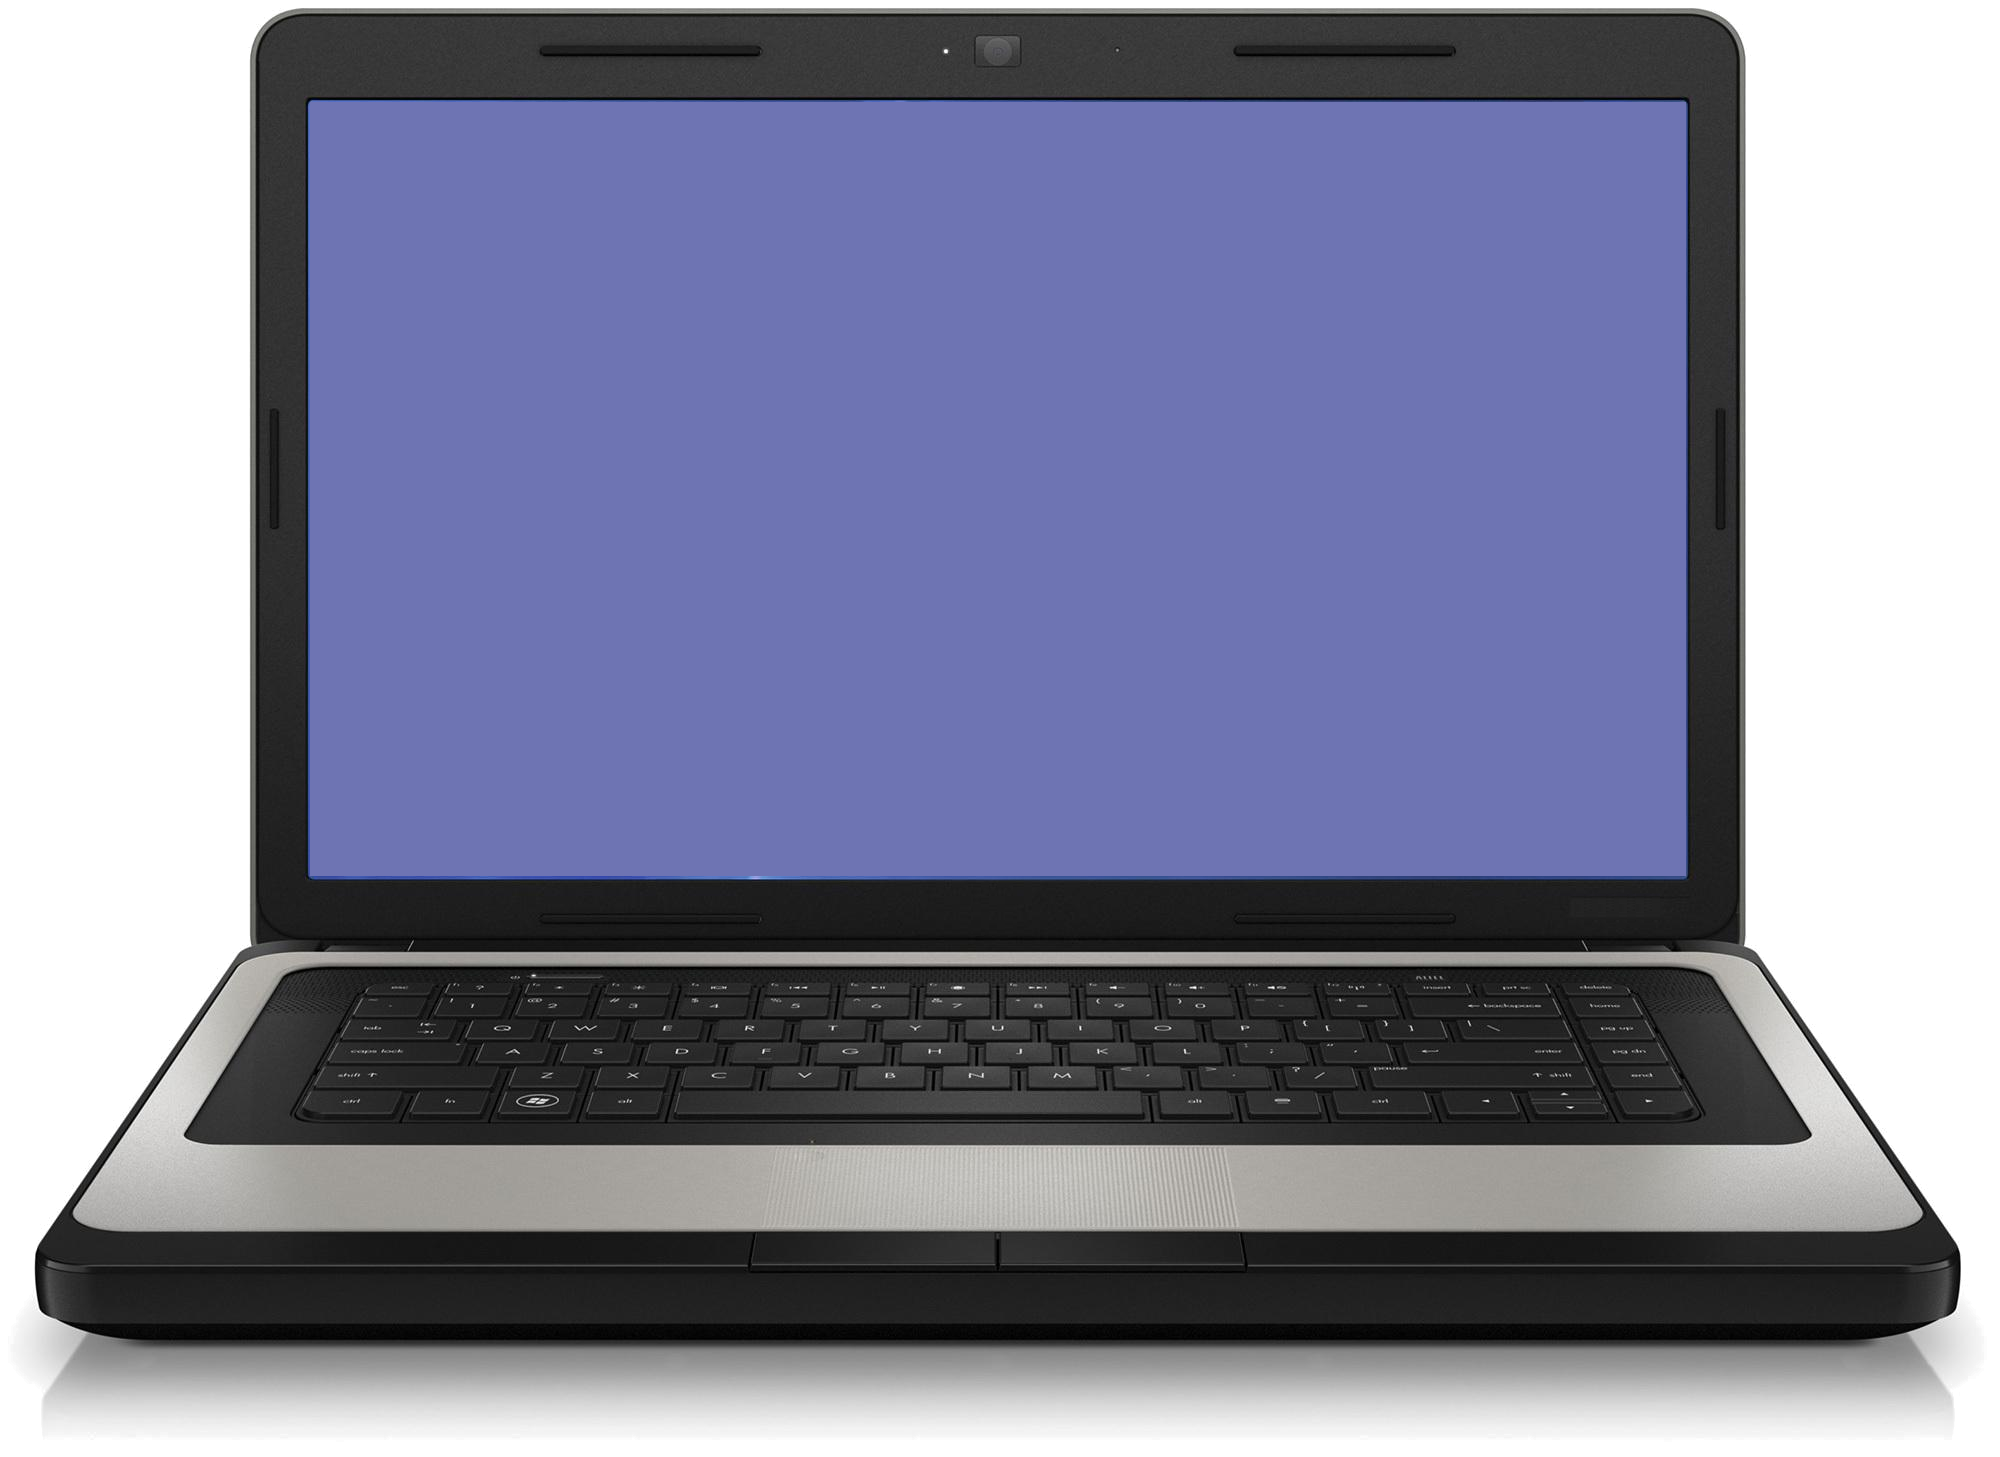
\includegraphics[width=0.6\linewidth]{figures/laptop.png}
           \end{textblock}                      
           \begin{textblock}{5}(9.5,2)
               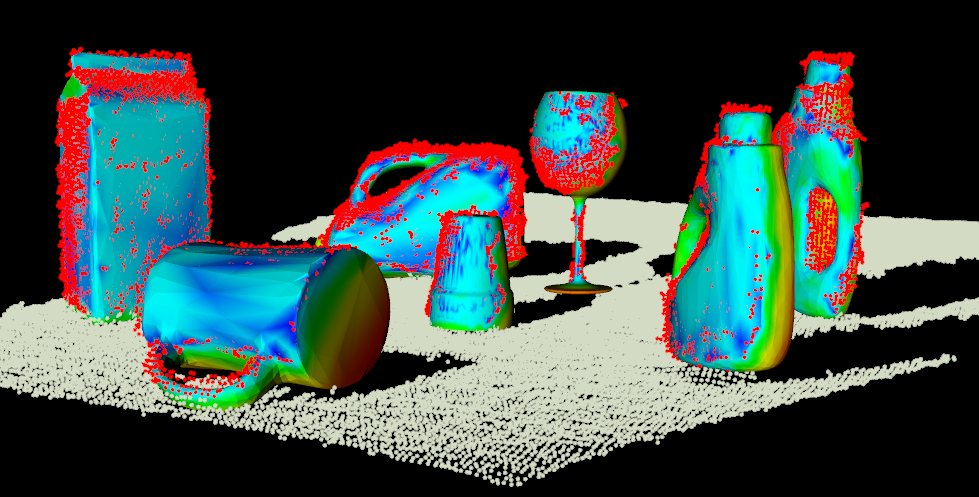
\includegraphics[width=1.0\linewidth]{figures/object_recognition.jpg}
              \end{textblock}       
       \end{frame} 
       
     \begin{frame}[plain]{}
         \begin{textblock}{5}(5,10)
             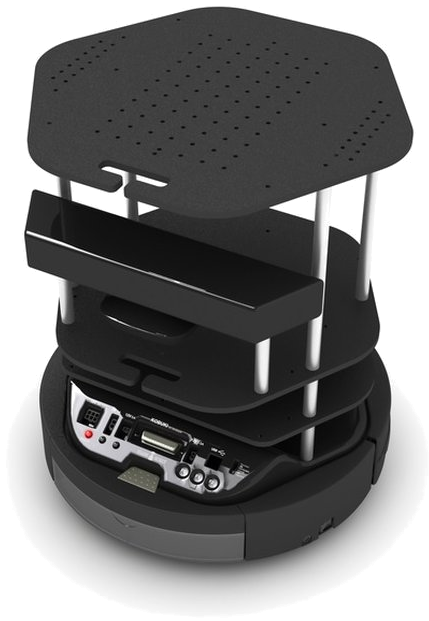
\includegraphics[width=0.5\linewidth]{figures/platform.png}
         \end{textblock}
         \begin{textblock}{5}(4,5.2)
             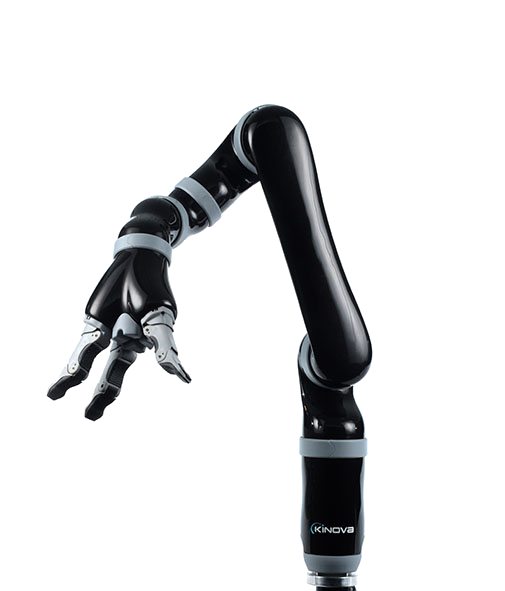
\includegraphics[width=0.7\linewidth]{figures/robot_arm.png}
         \end{textblock}
         \begin{textblock}{5}(5,1.5)
             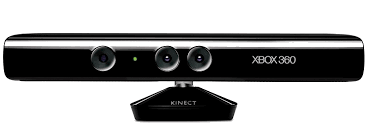
\includegraphics[width=0.6\linewidth]{figures/kinect.png}
         \end{textblock} 
         \begin{textblock}{5}(9.5,8)
             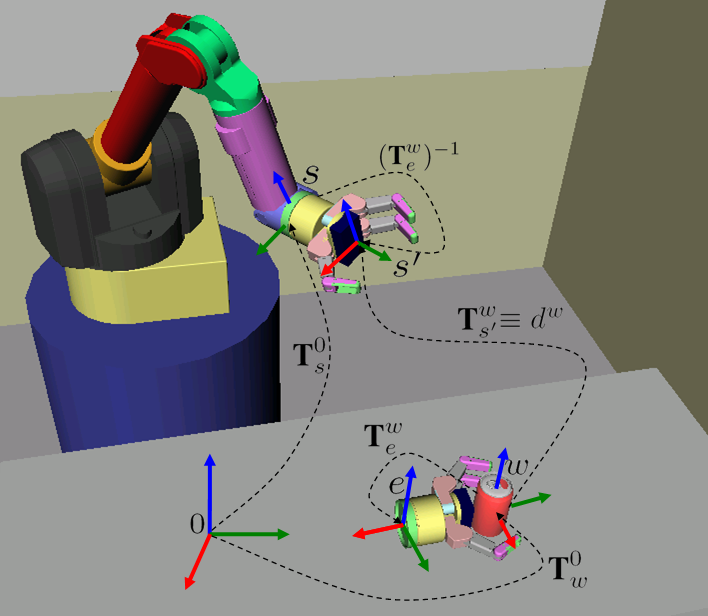
\includegraphics[width=1.2\linewidth]{figures/pick_and_place.png}
         \end{textblock}           
         \begin{textblock}{5}(0,5)
             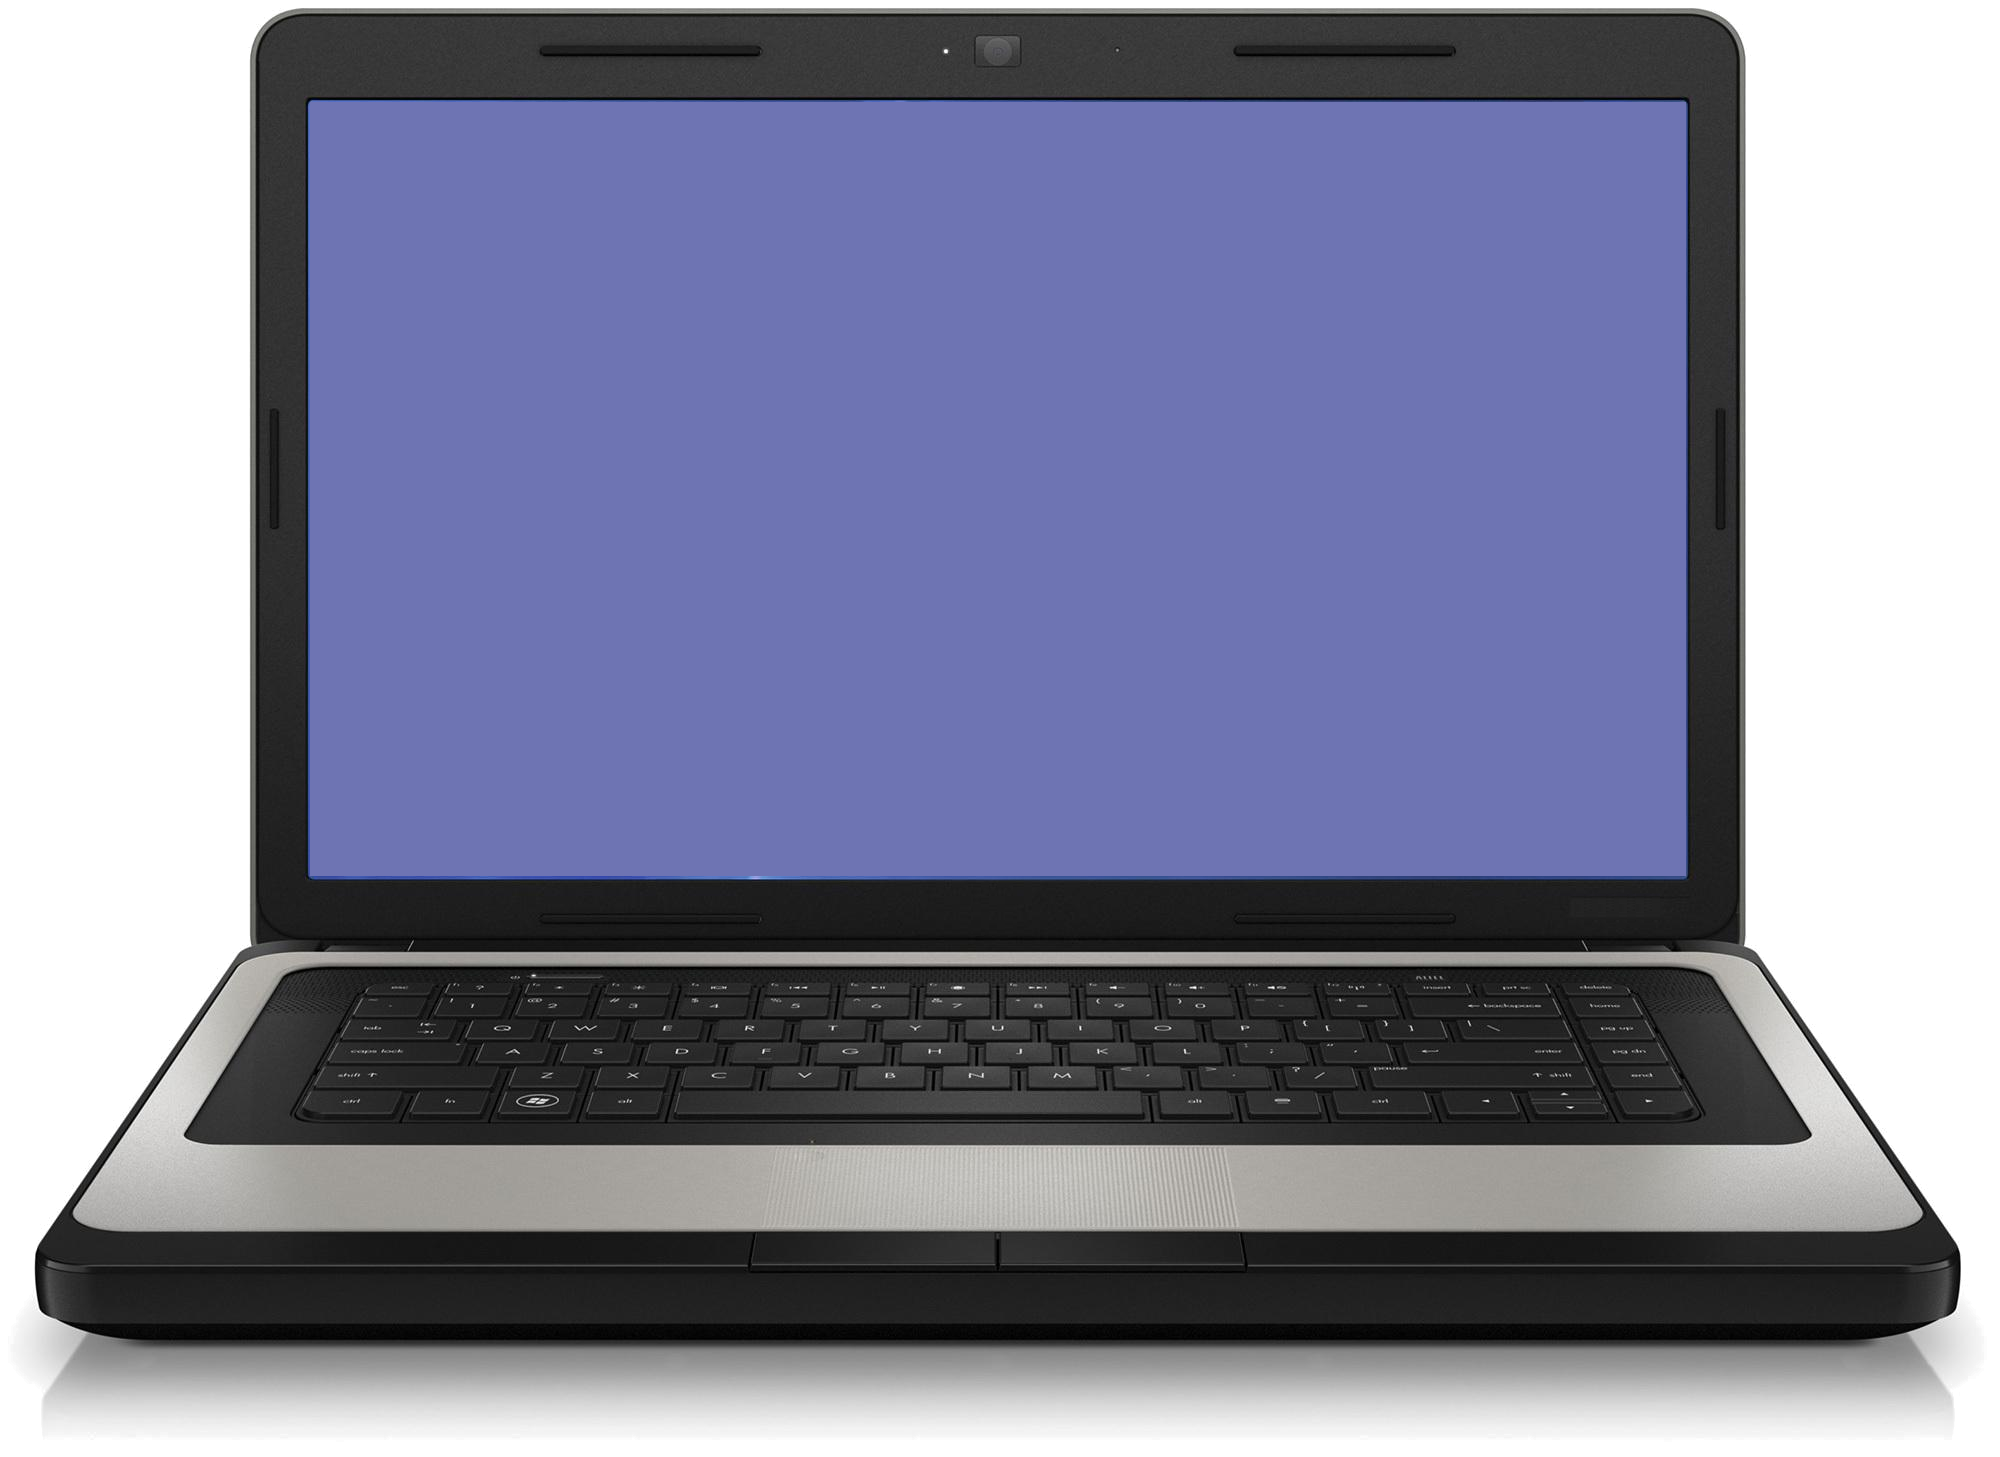
\includegraphics[width=0.6\linewidth]{figures/laptop.png}
         \end{textblock}                      
         \begin{textblock}{5}(9.5,2)
             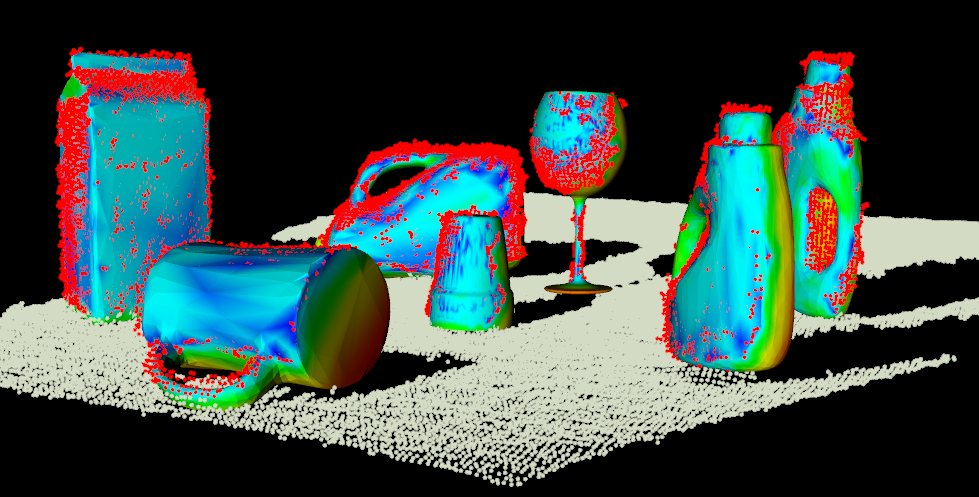
\includegraphics[width=1.0\linewidth]{figures/object_recognition.jpg}
         \end{textblock} 
         
         \begin{textblock}{5}(0.1,8)
        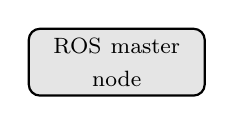
\begin{tikzpicture}
        \node [rectangle,draw,thick,text width=2.0cm,minimum height=0.7cm,
        text centered,rounded corners, fill=black!10] {\footnotesize ROS master node};
        \end{tikzpicture}
         \end{textblock} 

         \begin{textblock}{5}(5.1,3)
             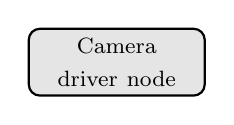
\begin{tikzpicture}
             \node [rectangle,draw,thick,text width=2.0cm,minimum height=0.7cm,
             text centered,rounded corners, fill=black!10] {\footnotesize Camera driver node};
             \end{tikzpicture}
            \end{textblock}
             
         \begin{textblock}{5}(6.5,7)
             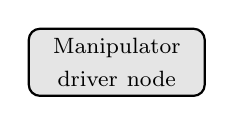
\begin{tikzpicture}
             \node [rectangle,draw,thick,text width=2.0cm,minimum height=0.7cm,
             text centered,rounded corners, fill=black!10] {\footnotesize Manipulator driver node};
             \end{tikzpicture}
            \end{textblock}  

         \begin{textblock}{5}(6.5,11)
             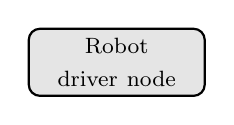
\begin{tikzpicture}
             \node [rectangle,draw,thick,text width=2.0cm,minimum height=0.7cm,
             text centered,rounded corners, fill=black!10] {\footnotesize Robot driver node};
             \end{tikzpicture}
         \end{textblock} 

         \begin{textblock}{5}(12,4)
             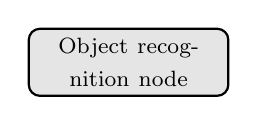
\begin{tikzpicture}
             \node [rectangle,draw,thick,text width=2.3cm,minimum height=0.7cm,
             text centered,rounded corners, fill=black!10] {\footnotesize Object recognition node};
             \end{tikzpicture}
           \end{textblock} 

         \begin{textblock}{5}(12.5,13.5)
             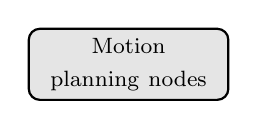
\begin{tikzpicture}
             \node [rectangle,draw,thick,text width=2.3cm,minimum height=0.7cm,
             text centered,rounded corners, fill=black!10] {\footnotesize Motion planning nodes};
             \end{tikzpicture}
            \end{textblock}                                                                     
     \end{frame}                            

\begin{frame}{Computation graph level}
    \framesubtitle{ROS Concepts}
    {\huge Topics and Messages:}
    \vspace{1cm}
    \begin{itemize}
        \item Nodes send data by publishing messages on a named topic.
        
        \item Nodes receive data by subscribing to a topic.
        
        \item Multiple nodes can publish/subscribe to the same topic.
        
        \item The publishing node and subscribing node are not aware of each other's existence. 
    \end{itemize}
\end{frame}

\begin{frame}{Computation graph level}
    \framesubtitle{ROS Concepts}
    {\huge Master:}
    \vspace{1cm}
    \begin{itemize}
        \item The first process to run in an application that uses ROS, is the Master.
        
        \item The ROS Master provides name registration and lookup to the rest
        of the nodes.
        
        \item In a distributed system, we should run the master on one computer,
        and other remote nodes can find each other by communicating with
        this master.
    \end{itemize}
\end{frame}

     \begin{frame}[plain]{}
     \centering
     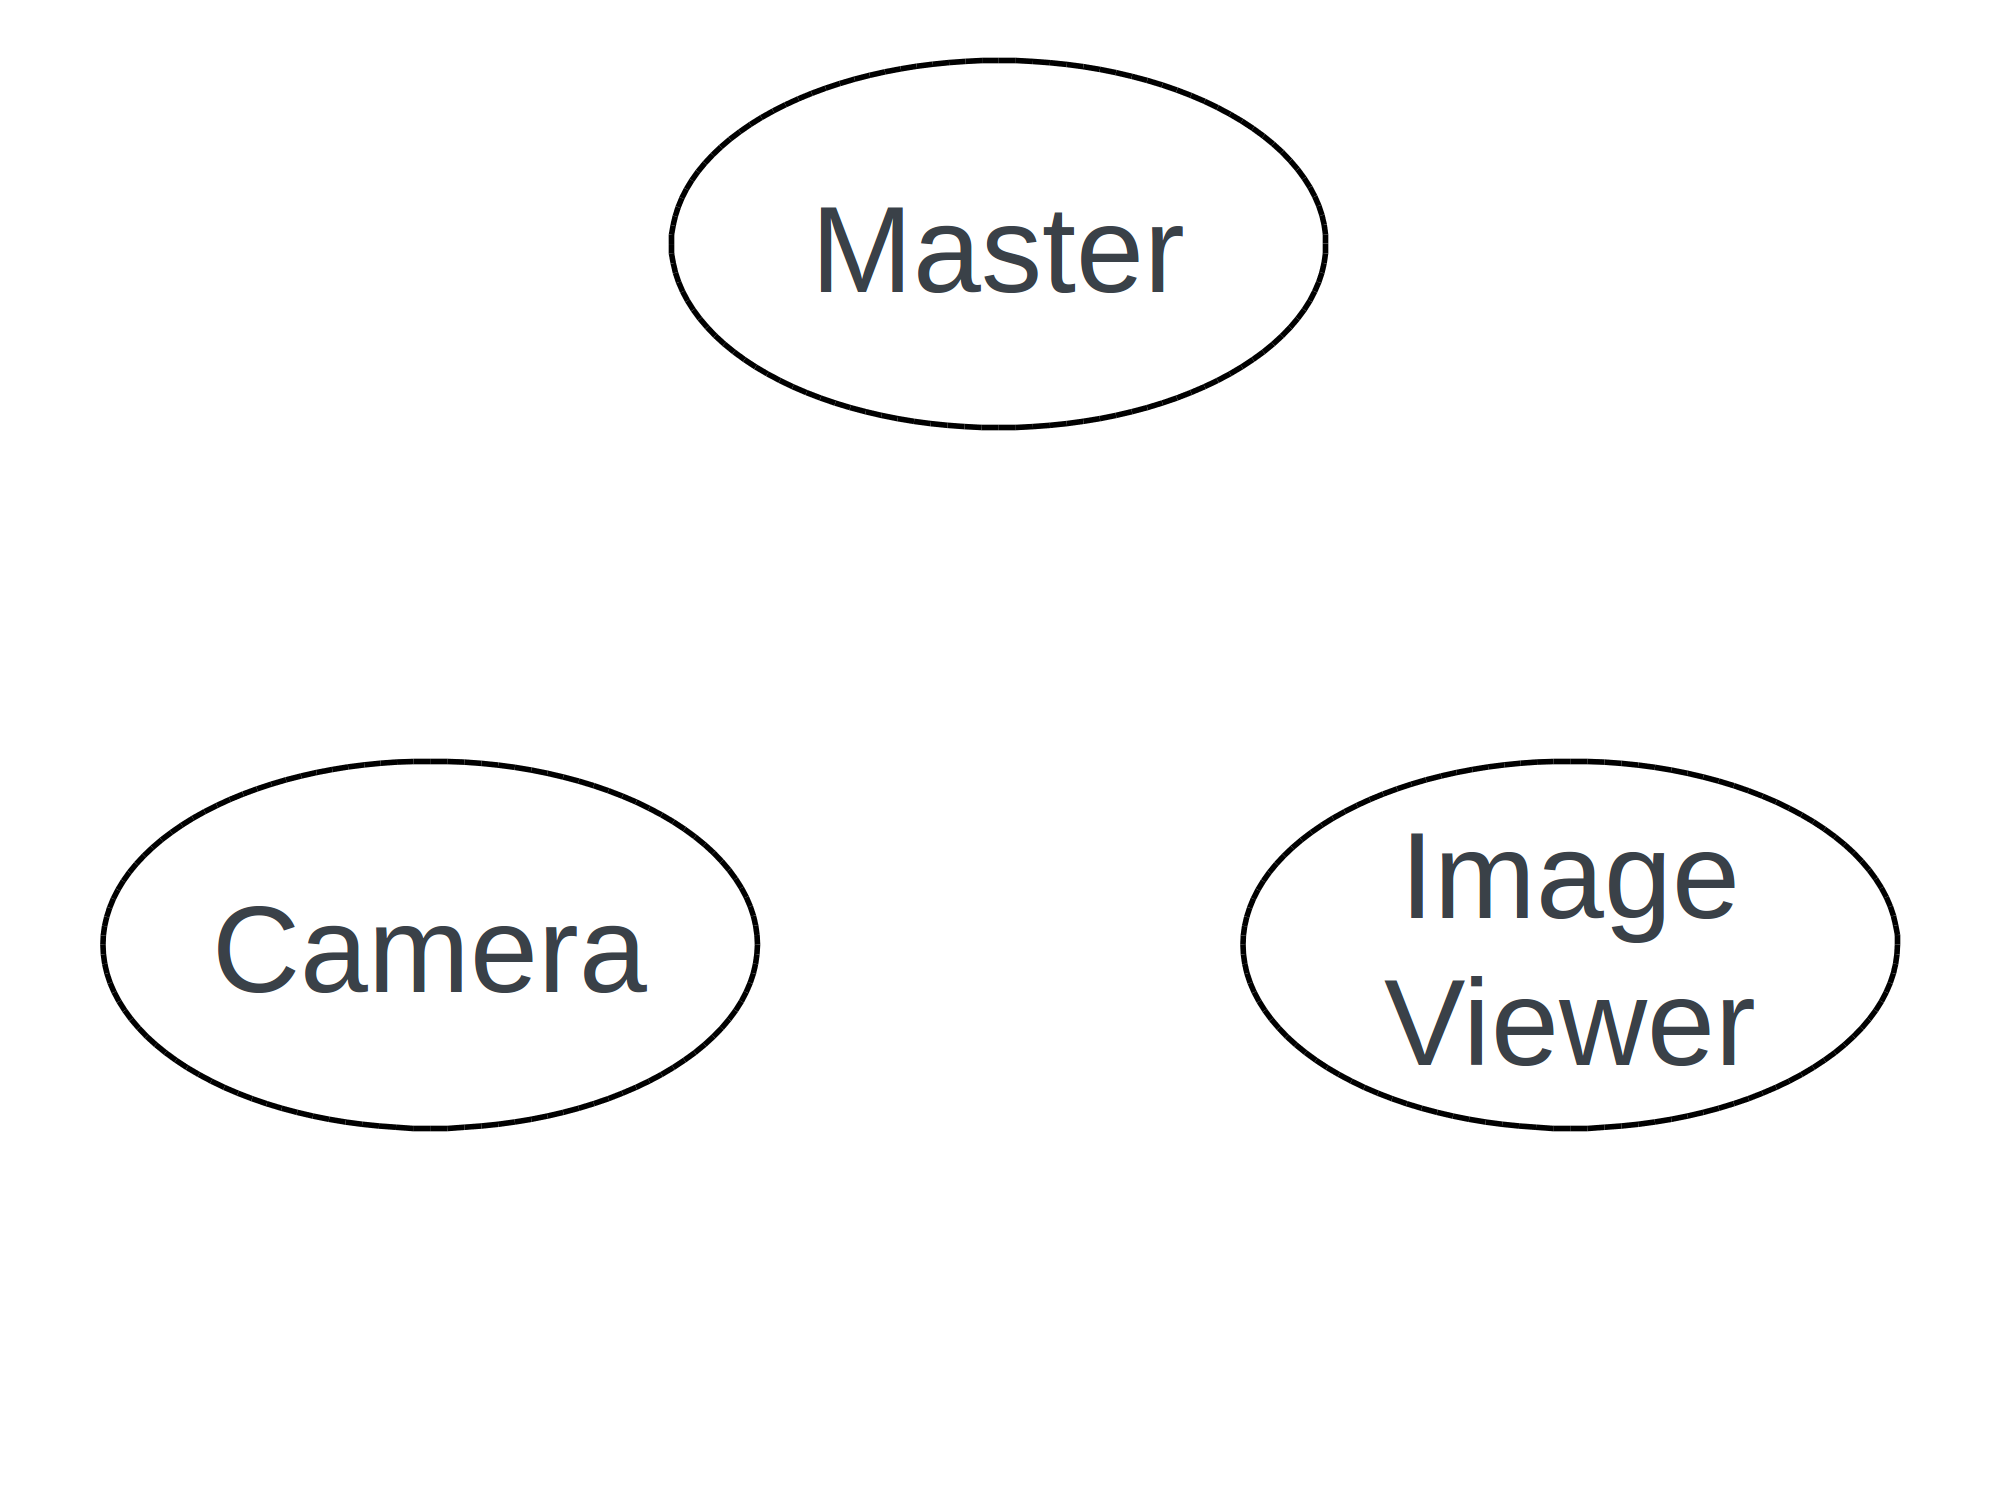
\includegraphics[width =1.0\linewidth]{figures/master1.png}                                                              
     \end{frame} 
     \begin{frame}[plain]{}
         \centering
         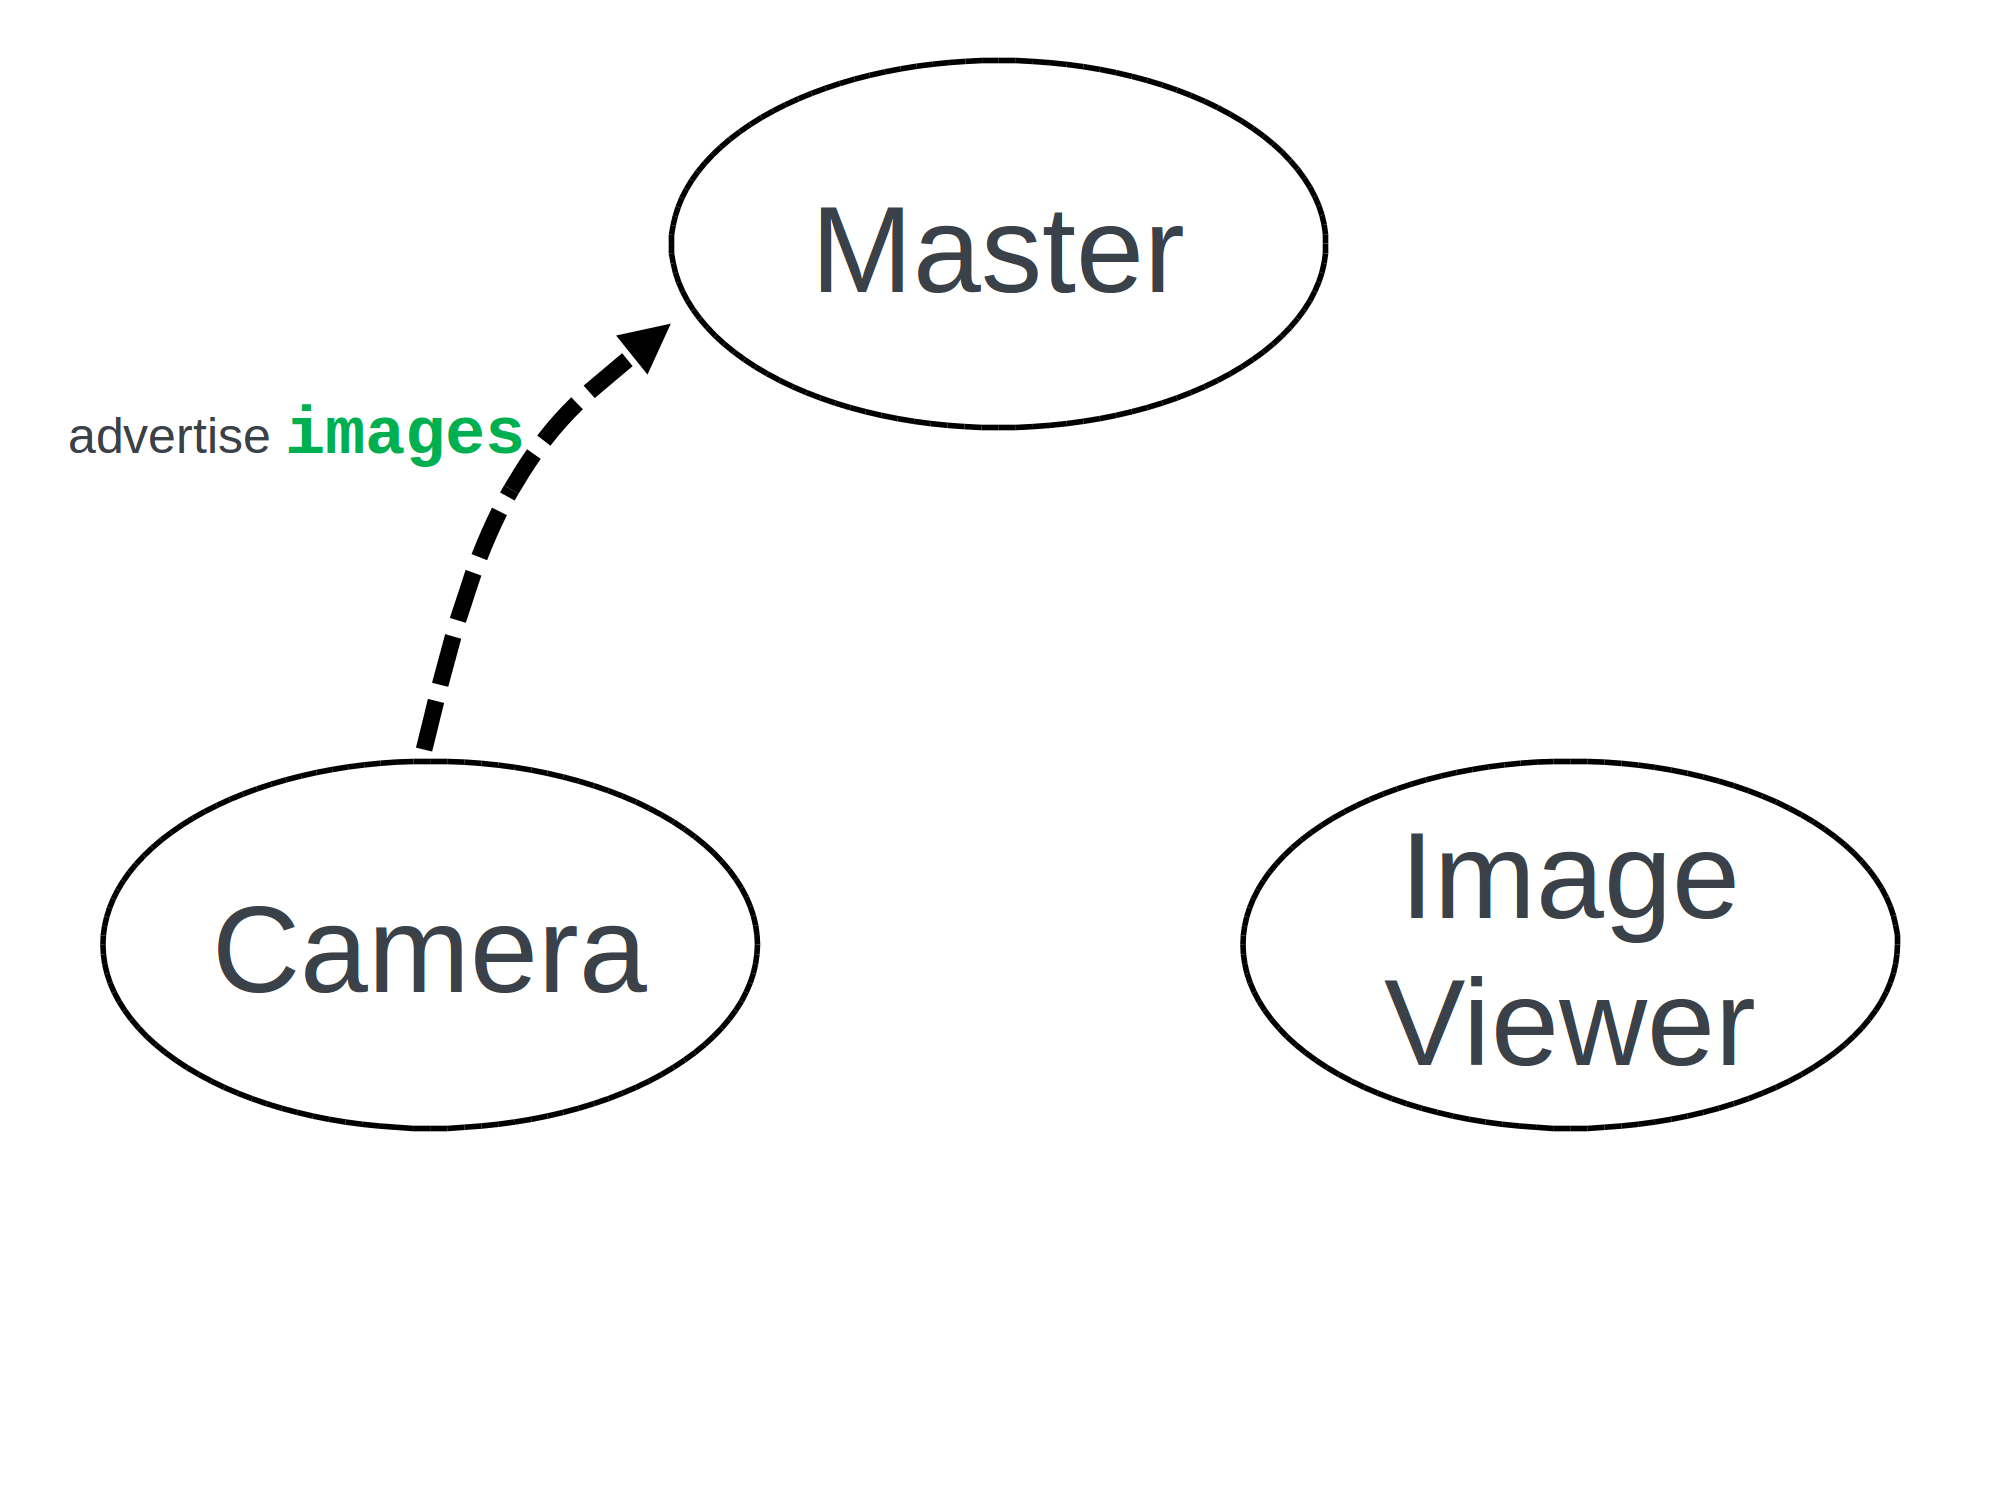
\includegraphics[width =1.0\linewidth]{figures/master2.png}                                                              
      \end{frame} 
     \begin{frame}[plain]{}
         \centering
         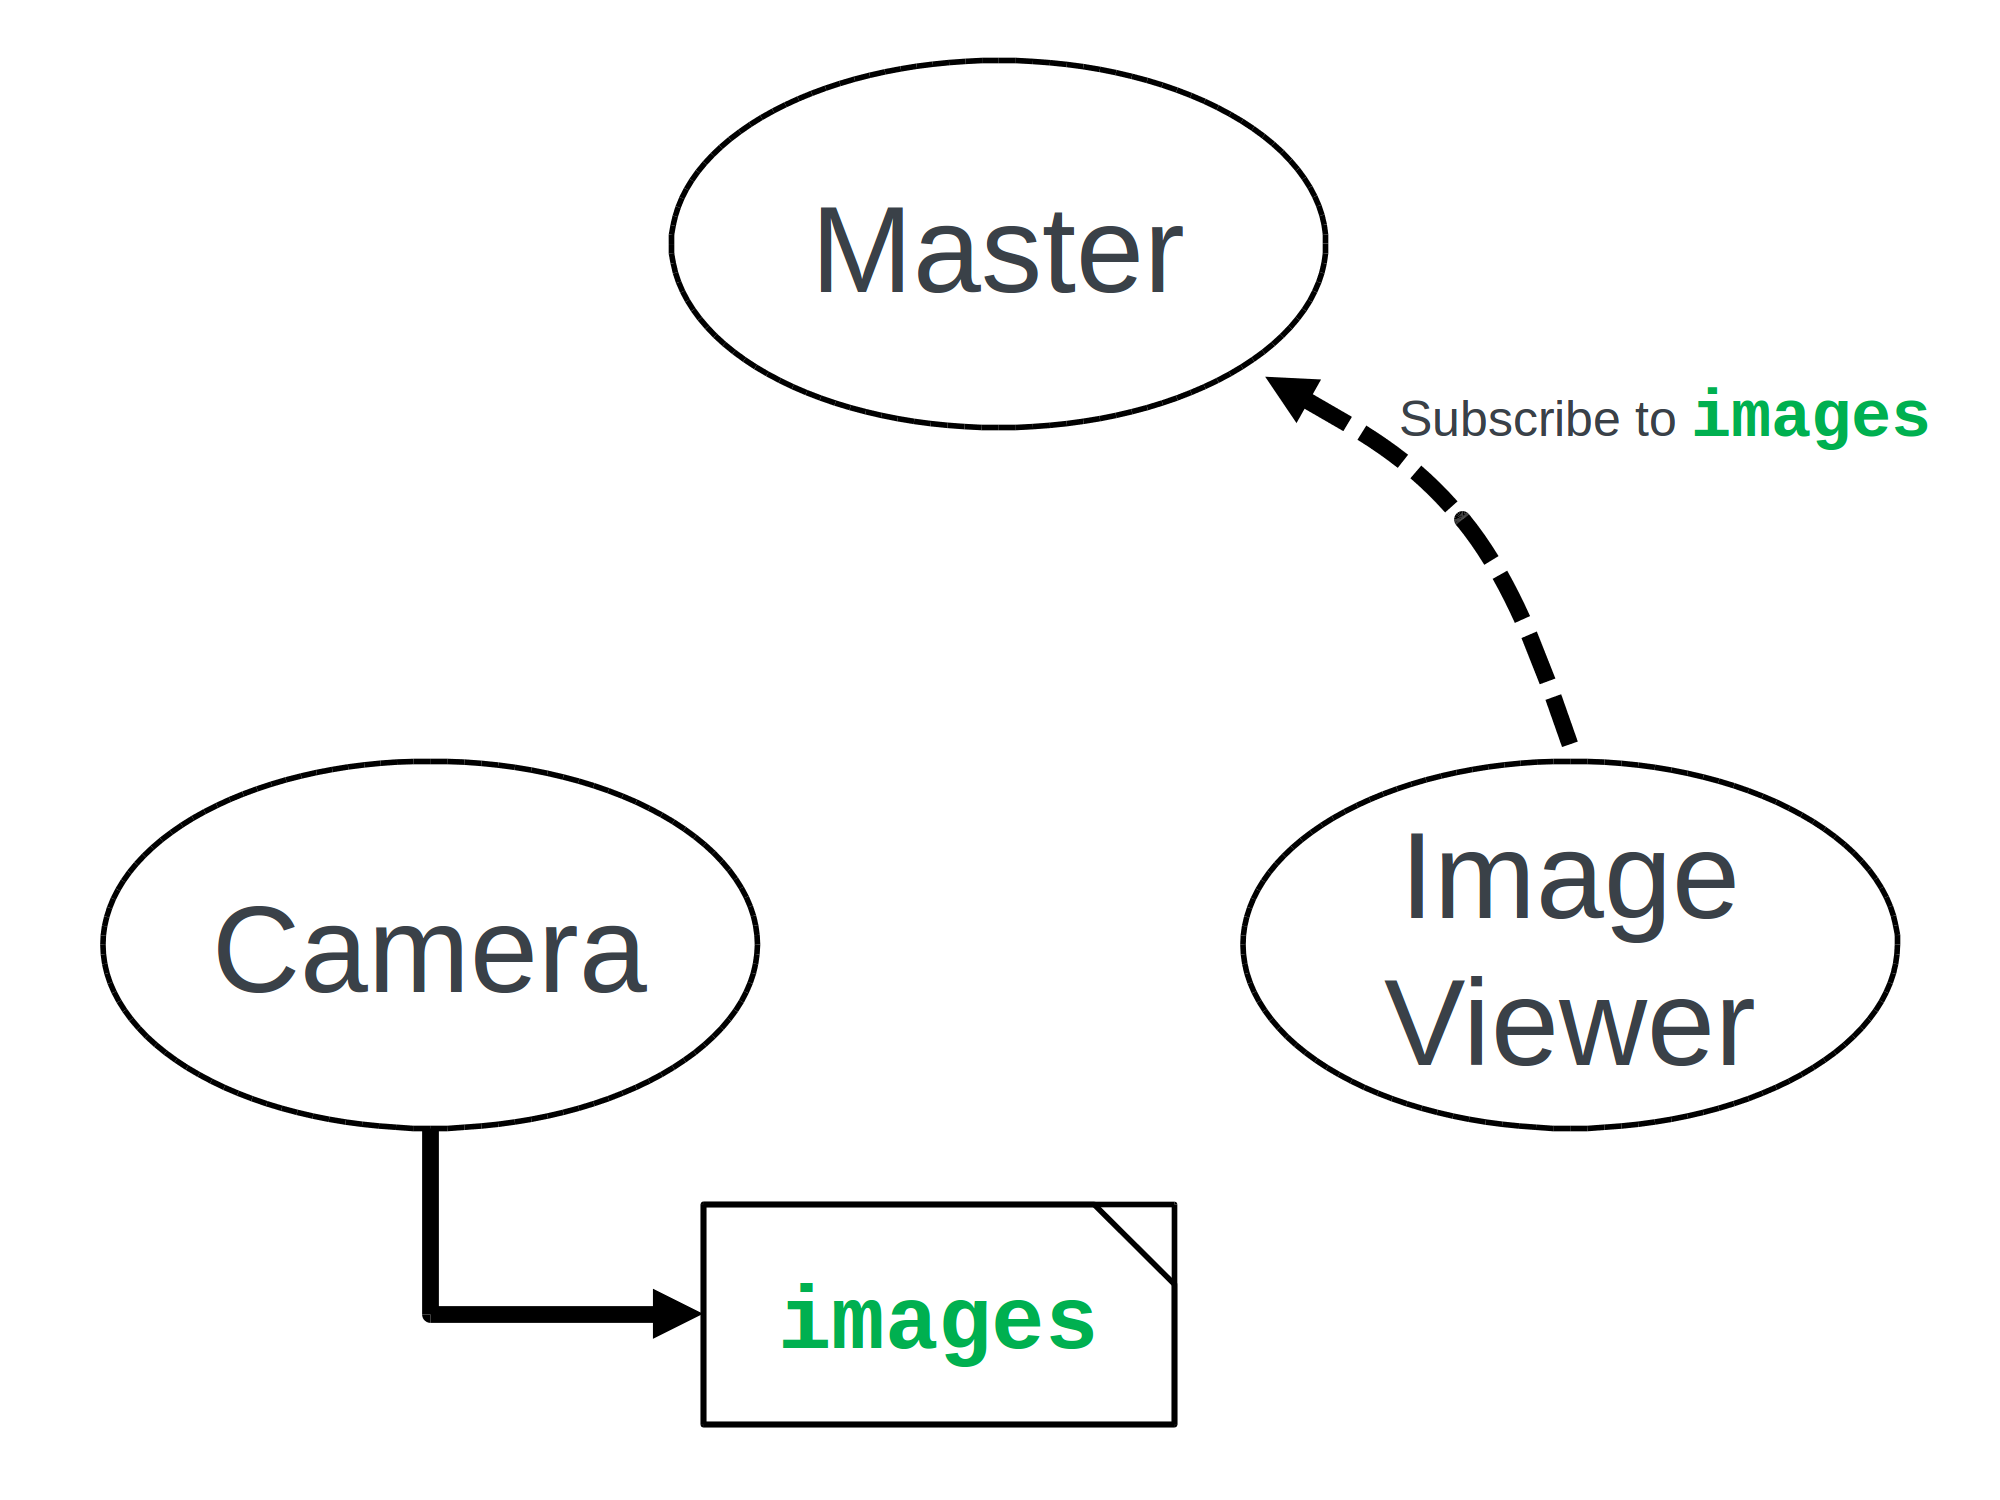
\includegraphics[width =1.0\linewidth]{figures/master3.png}                                                              
        \end{frame} 
     \begin{frame}[plain]{}
         \centering
         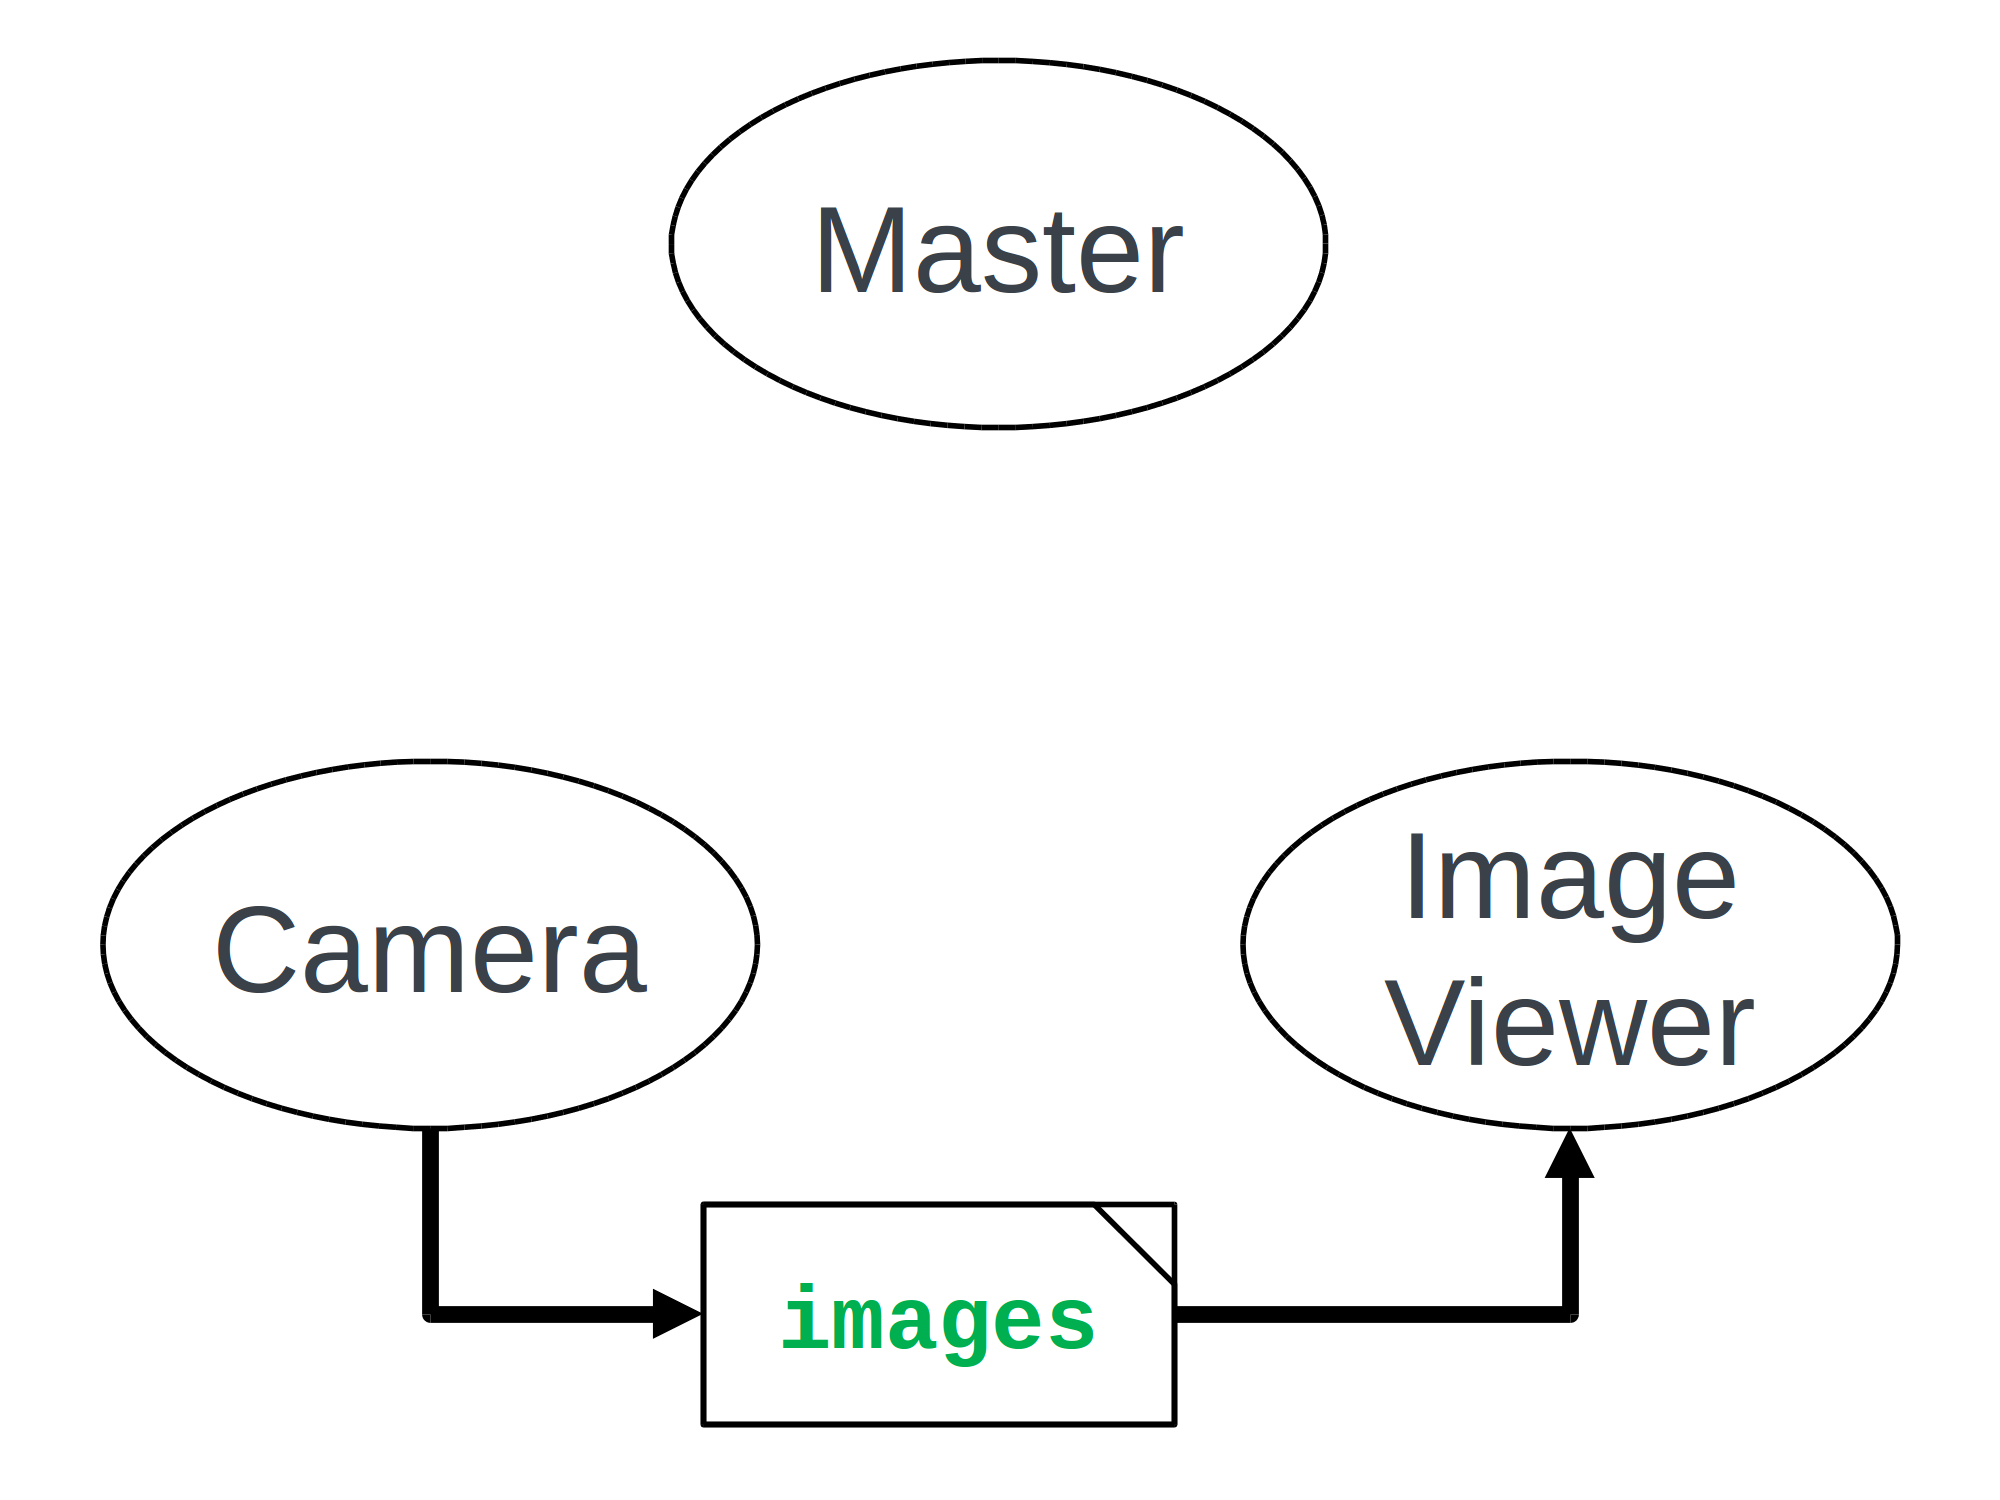
\includegraphics[width =1.0\linewidth]{figures/master4.png}                                                              
        \end{frame}
     \begin{frame}[plain]{}
         \centering
         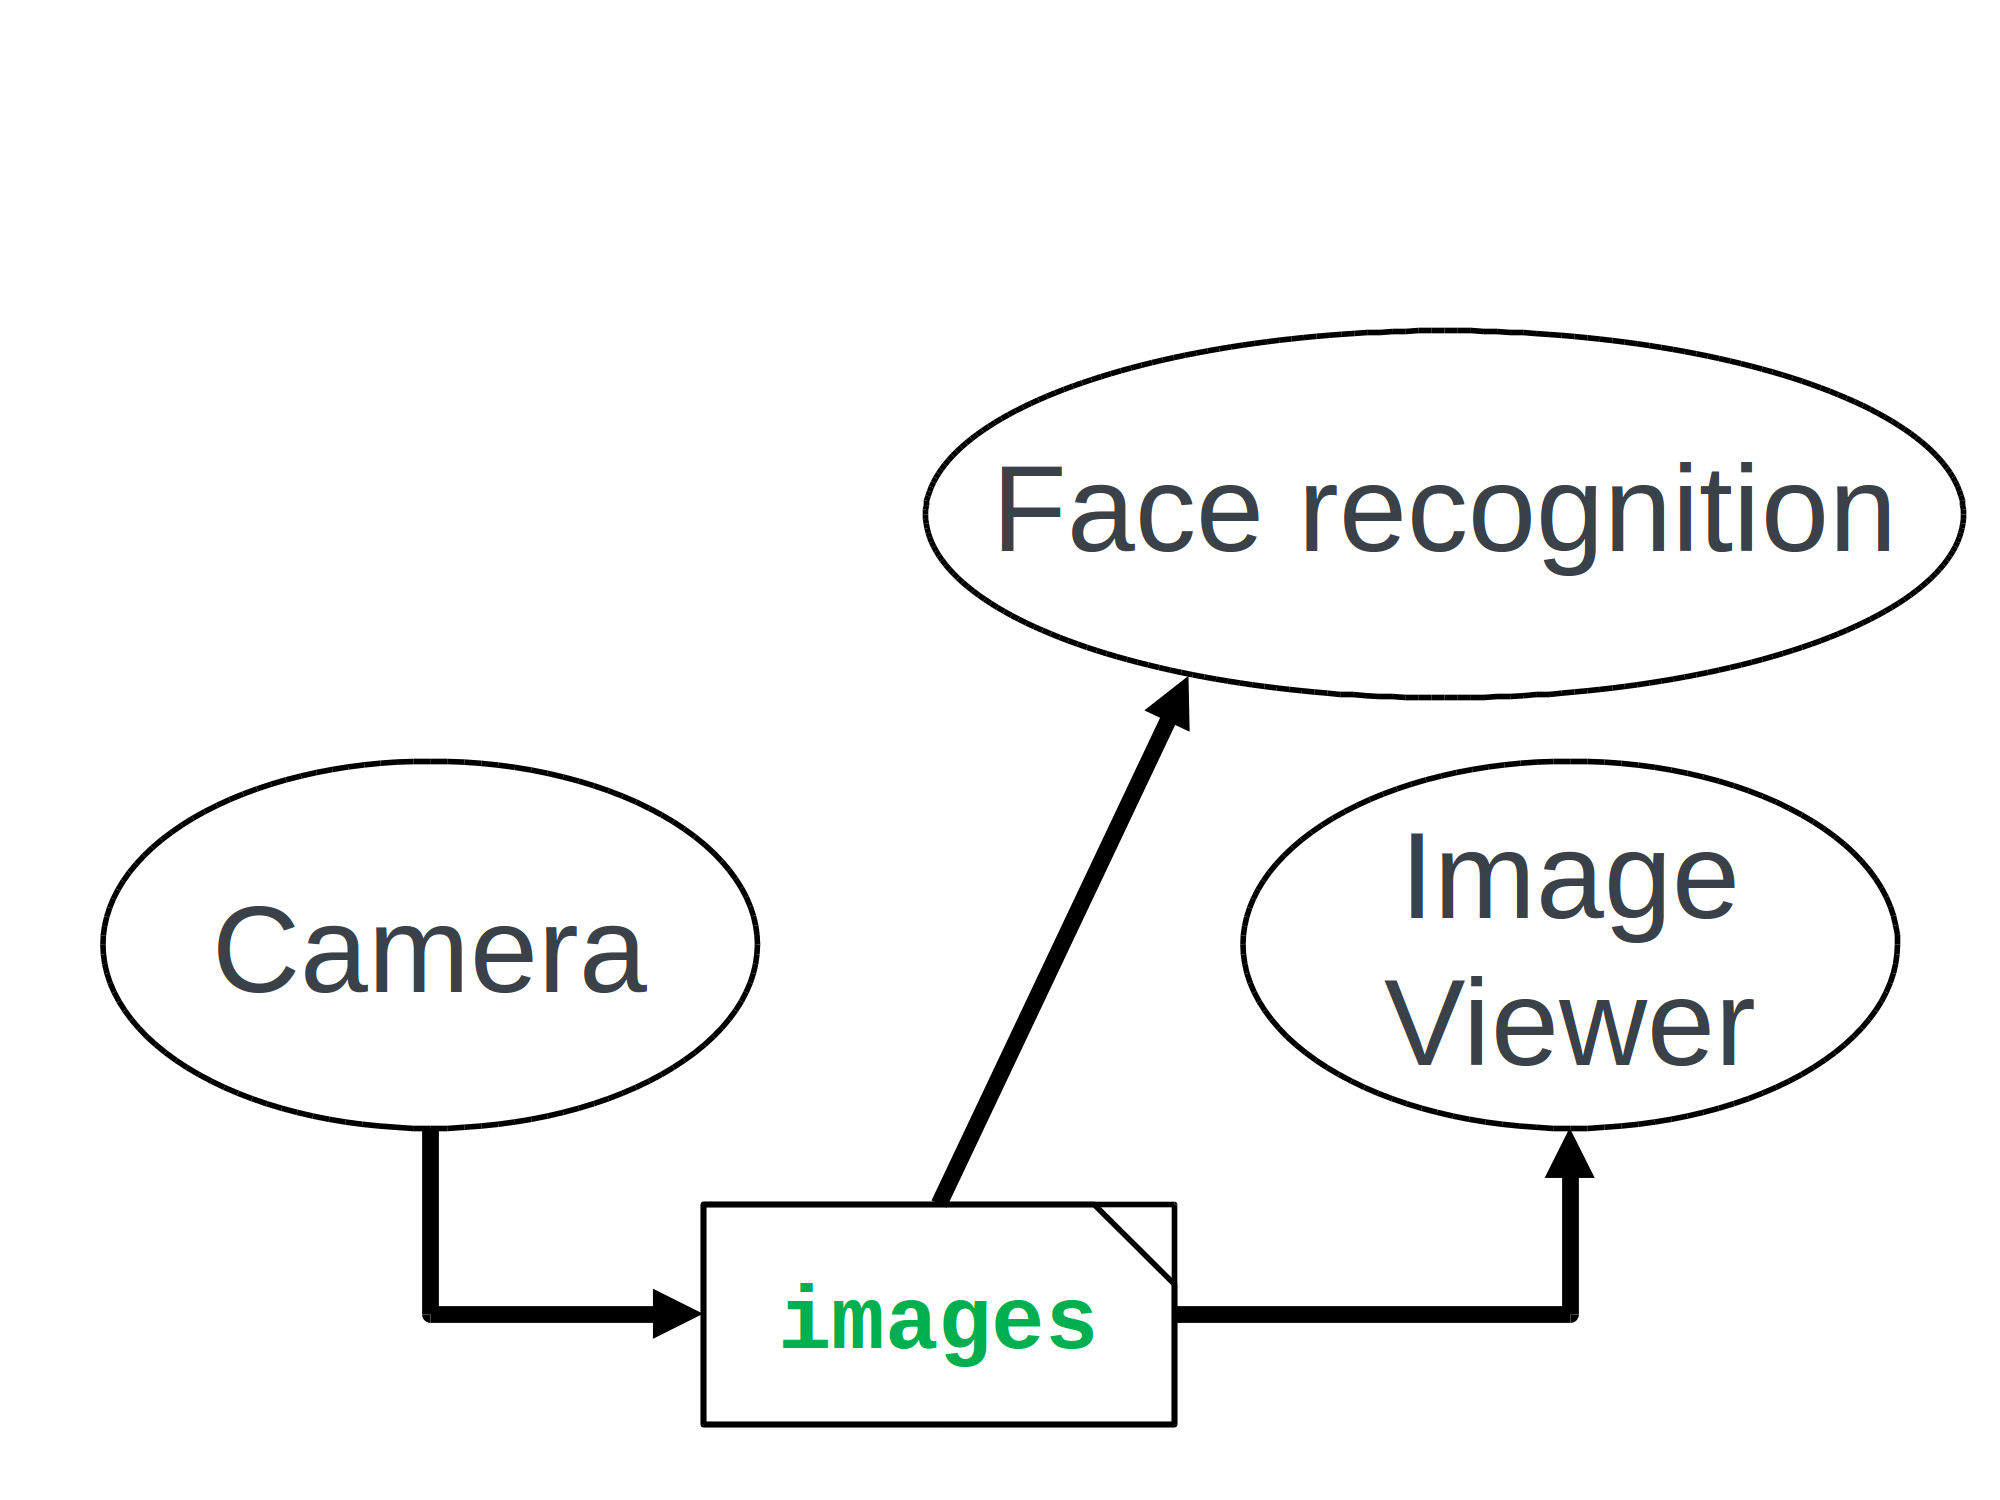
\includegraphics[width =1.0\linewidth]{figures/master5.png}                                                              
       \end{frame}                             

\begin{frame}{Computation graph level}
    \framesubtitle{ROS Concepts}
    {\huge Master:}
    \vspace{0.2cm}
    \begin{itemize}
        \item ROS master is invoked by this command:
    \end{itemize}
         \centering
         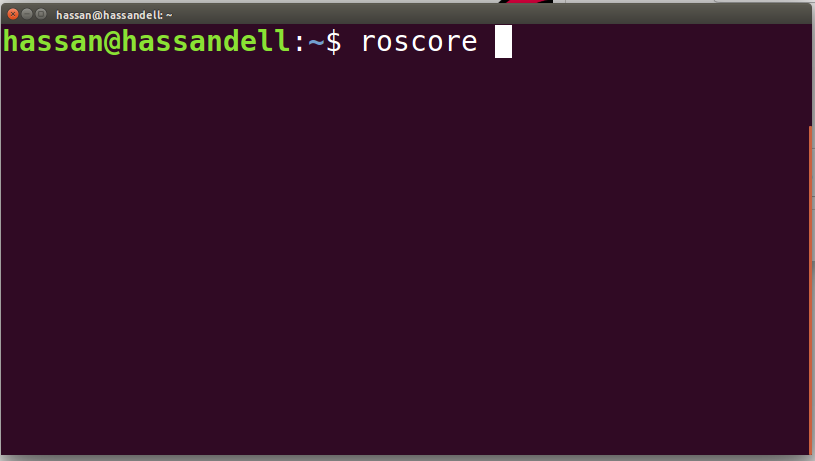
\includegraphics[width =0.75\linewidth]{figures/roscore.png}     
\end{frame}


\setbeamercolor{background canvas}{bg=black}
\begin{frame}[plain]{}  
    \centering
     {\huge \textcolor{white}{Example \\ (TurtleSim)} }
\end{frame}
\setbeamercolor{background canvas}{bg=white}

\begin{frame}{Computation graph level}
    \framesubtitle{ROS Concepts}
    
    Concepts related to ROS computation graph:
    
    \begin{enumerate}
        \item \textcolor{black!40}{Nodes.}
        \item \textcolor{black!40}{Topics.}
        \item \textcolor{black!40}{Messages.}
        \item \textcolor{black!40}{Master.}
        \item Parameter Server.
        \item Services.
        \item Bags.
    \end{enumerate}
\end{frame}

\begin{frame}{Computation graph level}
    \framesubtitle{ROS Concepts}
    {\huge Parameter Server:}
    \vspace{0.2cm}
    \begin{itemize}
        \item A network-shared dictionary accessible to all nodes.
        \item Typically used to store static data, like parameters and configurations.
        \item A central location to store static values.
        \item  All nodes can access and modify those values.
        \item Parameter server is a part of ROS Master.
    \end{itemize}  
\end{frame}

\begin{frame}{Computation graph level}
    \framesubtitle{ROS Concepts}
    {\huge Services:}
    \vspace{0.2cm}
    \begin{itemize}
        \item Sometimes a publish/subscribe model is not enough, it’s a one-way
        communication.
        \item ROS Services provide an additional way of interaction, a  \textbf{request / reply}
        interaction.
    \end{itemize}  
\end{frame}

\begin{frame}{Computation graph level}
    \framesubtitle{ROS Concepts}
    {\huge Bags:}
    \vspace{0.2cm}
    \begin{itemize}
        \item ROS bag is a mechanism for recording data for later playback.
        \item You can record a complete session, with all the topics and messages
        being exchanged along with their time stamping.
    \end{itemize}  
\end{frame}
    
\subsection{Community level}
\begin{frame}{Community level}
    \framesubtitle{ROS Concepts}
    
    Concepts related to ROS development process and it's community:
    
    \begin{enumerate}
        \item ROS Distributions.
        \item The ROS Wiki.
        \item Mailing Lists.
        \item ROS Answers.
    \end{enumerate}
\end{frame}


\begin{frame}{Community level}
    \framesubtitle{ROS Concepts}
    {\huge ROS Distributions:}
    \vspace{7.0cm}
     \begin{textblock}{3}(1,5)
        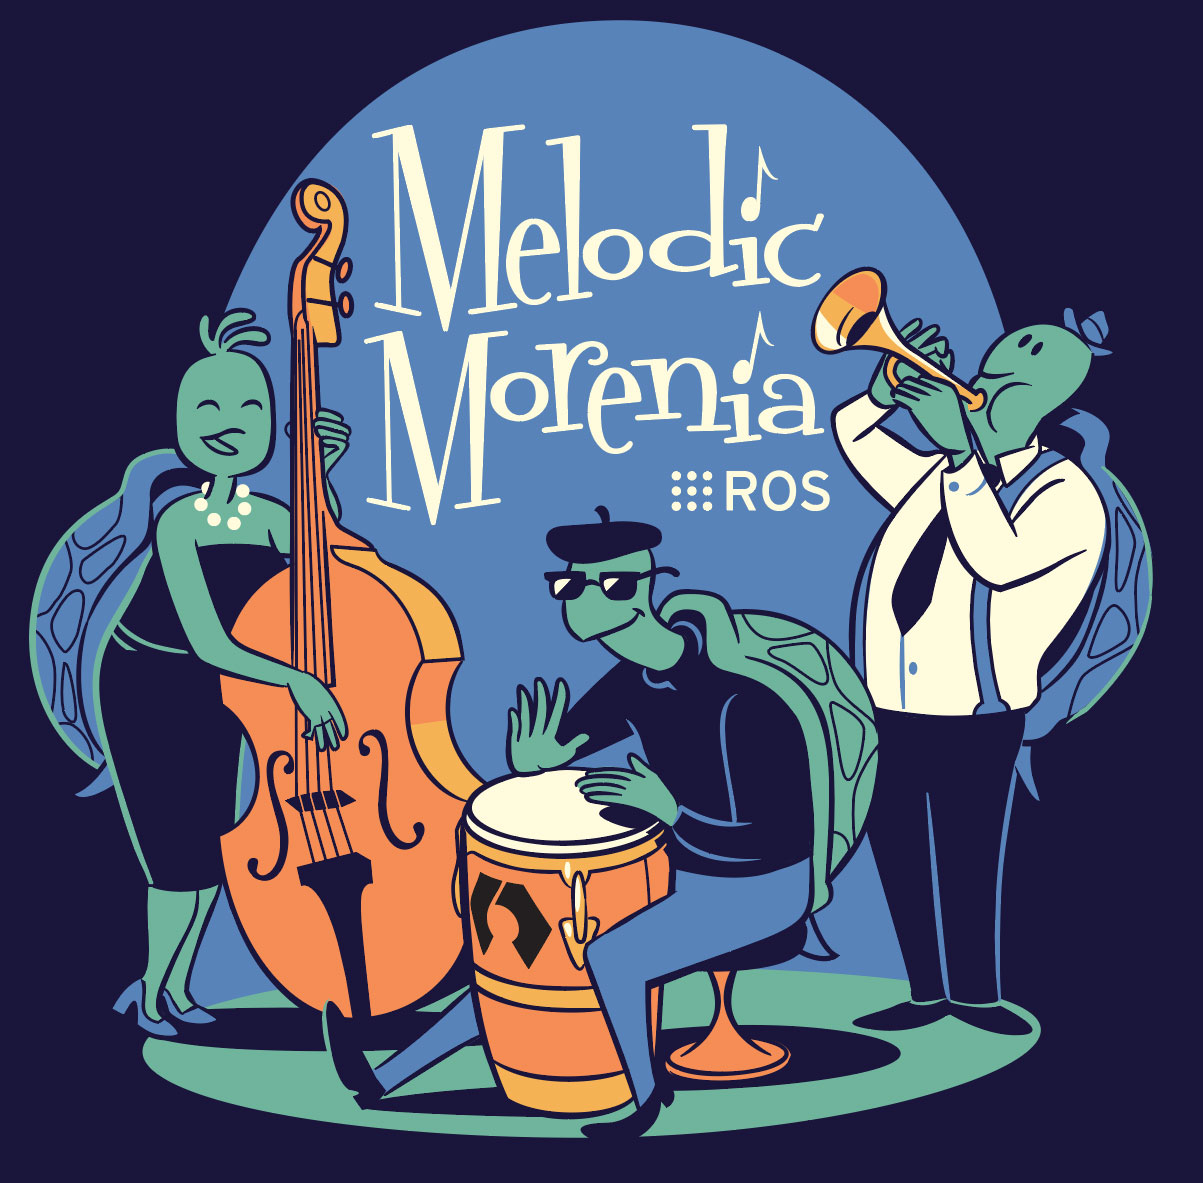
\includegraphics[width = 1.0\linewidth]{figures/melodic.jpg}
        
        \centering
        ROS Melodic\\
        \footnotesize 5.2018 - 5.2023\\
        (LTS)\\
        (Ubuntu 18 EOL)
        
     \end{textblock}
     \begin{textblock}{3}(4.5,5)
         
\includegraphics[width = 1.0\linewidth]{figures/lunar.png}
         
         \centering
         ROS Lunar\\
         \footnotesize 5.2017 - 4.2019
     \end{textblock}
     \begin{textblock}{3}(8,5)
         
\includegraphics[width = 1.0\linewidth]{figures/kinetic.png}
         
         \centering
         ROS Kinetic\\
         \footnotesize 5.2016 - 4.2021\\
         (LTS)\\
         (Ubuntu 16 EOL)\\
         (what we use)
         
     \end{textblock}  
     \begin{textblock}{3}(11.5,5)
         
\includegraphics[width = 1.0\linewidth]{figures/indigo.png}
         
         \centering
         ROS Indigo\\
         \footnotesize 7.2014 - 4.2019\\
         (LTS)\\
         (Ubuntu 14 EOL)\\
     \end{textblock}                       
\end{frame}

\setbeamercolor{background canvas}{bg=black}
\begin{frame}[plain]{}  
    \centering
    {\huge \textcolor{white}{Thank you}}
    
    \vspace{0.5cm}
    
    {\huge \textcolor{white}{Any questions?}}
\end{frame}
\setbeamercolor{background canvas}{bg=white}


\end{document}
